% Options for packages loaded elsewhere
\PassOptionsToPackage{unicode}{hyperref}
\PassOptionsToPackage{hyphens}{url}
\PassOptionsToPackage{dvipsnames,svgnames,x11names}{xcolor}
%
\documentclass[
  letterpaper,
  DIV=11,
  numbers=noendperiod]{scrreprt}

\usepackage{amsmath,amssymb}
\usepackage{iftex}
\ifPDFTeX
  \usepackage[T1]{fontenc}
  \usepackage[utf8]{inputenc}
  \usepackage{textcomp} % provide euro and other symbols
\else % if luatex or xetex
  \usepackage{unicode-math}
  \defaultfontfeatures{Scale=MatchLowercase}
  \defaultfontfeatures[\rmfamily]{Ligatures=TeX,Scale=1}
\fi
\usepackage{lmodern}
\ifPDFTeX\else  
    % xetex/luatex font selection
\fi
% Use upquote if available, for straight quotes in verbatim environments
\IfFileExists{upquote.sty}{\usepackage{upquote}}{}
\IfFileExists{microtype.sty}{% use microtype if available
  \usepackage[]{microtype}
  \UseMicrotypeSet[protrusion]{basicmath} % disable protrusion for tt fonts
}{}
\makeatletter
\@ifundefined{KOMAClassName}{% if non-KOMA class
  \IfFileExists{parskip.sty}{%
    \usepackage{parskip}
  }{% else
    \setlength{\parindent}{0pt}
    \setlength{\parskip}{6pt plus 2pt minus 1pt}}
}{% if KOMA class
  \KOMAoptions{parskip=half}}
\makeatother
\usepackage{xcolor}
\setlength{\emergencystretch}{3em} % prevent overfull lines
\setcounter{secnumdepth}{5}
% Make \paragraph and \subparagraph free-standing
\ifx\paragraph\undefined\else
  \let\oldparagraph\paragraph
  \renewcommand{\paragraph}[1]{\oldparagraph{#1}\mbox{}}
\fi
\ifx\subparagraph\undefined\else
  \let\oldsubparagraph\subparagraph
  \renewcommand{\subparagraph}[1]{\oldsubparagraph{#1}\mbox{}}
\fi

\usepackage{color}
\usepackage{fancyvrb}
\newcommand{\VerbBar}{|}
\newcommand{\VERB}{\Verb[commandchars=\\\{\}]}
\DefineVerbatimEnvironment{Highlighting}{Verbatim}{commandchars=\\\{\}}
% Add ',fontsize=\small' for more characters per line
\usepackage{framed}
\definecolor{shadecolor}{RGB}{241,243,245}
\newenvironment{Shaded}{\begin{snugshade}}{\end{snugshade}}
\newcommand{\AlertTok}[1]{\textcolor[rgb]{0.68,0.00,0.00}{#1}}
\newcommand{\AnnotationTok}[1]{\textcolor[rgb]{0.37,0.37,0.37}{#1}}
\newcommand{\AttributeTok}[1]{\textcolor[rgb]{0.40,0.45,0.13}{#1}}
\newcommand{\BaseNTok}[1]{\textcolor[rgb]{0.68,0.00,0.00}{#1}}
\newcommand{\BuiltInTok}[1]{\textcolor[rgb]{0.00,0.23,0.31}{#1}}
\newcommand{\CharTok}[1]{\textcolor[rgb]{0.13,0.47,0.30}{#1}}
\newcommand{\CommentTok}[1]{\textcolor[rgb]{0.37,0.37,0.37}{#1}}
\newcommand{\CommentVarTok}[1]{\textcolor[rgb]{0.37,0.37,0.37}{\textit{#1}}}
\newcommand{\ConstantTok}[1]{\textcolor[rgb]{0.56,0.35,0.01}{#1}}
\newcommand{\ControlFlowTok}[1]{\textcolor[rgb]{0.00,0.23,0.31}{#1}}
\newcommand{\DataTypeTok}[1]{\textcolor[rgb]{0.68,0.00,0.00}{#1}}
\newcommand{\DecValTok}[1]{\textcolor[rgb]{0.68,0.00,0.00}{#1}}
\newcommand{\DocumentationTok}[1]{\textcolor[rgb]{0.37,0.37,0.37}{\textit{#1}}}
\newcommand{\ErrorTok}[1]{\textcolor[rgb]{0.68,0.00,0.00}{#1}}
\newcommand{\ExtensionTok}[1]{\textcolor[rgb]{0.00,0.23,0.31}{#1}}
\newcommand{\FloatTok}[1]{\textcolor[rgb]{0.68,0.00,0.00}{#1}}
\newcommand{\FunctionTok}[1]{\textcolor[rgb]{0.28,0.35,0.67}{#1}}
\newcommand{\ImportTok}[1]{\textcolor[rgb]{0.00,0.46,0.62}{#1}}
\newcommand{\InformationTok}[1]{\textcolor[rgb]{0.37,0.37,0.37}{#1}}
\newcommand{\KeywordTok}[1]{\textcolor[rgb]{0.00,0.23,0.31}{#1}}
\newcommand{\NormalTok}[1]{\textcolor[rgb]{0.00,0.23,0.31}{#1}}
\newcommand{\OperatorTok}[1]{\textcolor[rgb]{0.37,0.37,0.37}{#1}}
\newcommand{\OtherTok}[1]{\textcolor[rgb]{0.00,0.23,0.31}{#1}}
\newcommand{\PreprocessorTok}[1]{\textcolor[rgb]{0.68,0.00,0.00}{#1}}
\newcommand{\RegionMarkerTok}[1]{\textcolor[rgb]{0.00,0.23,0.31}{#1}}
\newcommand{\SpecialCharTok}[1]{\textcolor[rgb]{0.37,0.37,0.37}{#1}}
\newcommand{\SpecialStringTok}[1]{\textcolor[rgb]{0.13,0.47,0.30}{#1}}
\newcommand{\StringTok}[1]{\textcolor[rgb]{0.13,0.47,0.30}{#1}}
\newcommand{\VariableTok}[1]{\textcolor[rgb]{0.07,0.07,0.07}{#1}}
\newcommand{\VerbatimStringTok}[1]{\textcolor[rgb]{0.13,0.47,0.30}{#1}}
\newcommand{\WarningTok}[1]{\textcolor[rgb]{0.37,0.37,0.37}{\textit{#1}}}

\providecommand{\tightlist}{%
  \setlength{\itemsep}{0pt}\setlength{\parskip}{0pt}}\usepackage{longtable,booktabs,array}
\usepackage{calc} % for calculating minipage widths
% Correct order of tables after \paragraph or \subparagraph
\usepackage{etoolbox}
\makeatletter
\patchcmd\longtable{\par}{\if@noskipsec\mbox{}\fi\par}{}{}
\makeatother
% Allow footnotes in longtable head/foot
\IfFileExists{footnotehyper.sty}{\usepackage{footnotehyper}}{\usepackage{footnote}}
\makesavenoteenv{longtable}
\usepackage{graphicx}
\makeatletter
\def\maxwidth{\ifdim\Gin@nat@width>\linewidth\linewidth\else\Gin@nat@width\fi}
\def\maxheight{\ifdim\Gin@nat@height>\textheight\textheight\else\Gin@nat@height\fi}
\makeatother
% Scale images if necessary, so that they will not overflow the page
% margins by default, and it is still possible to overwrite the defaults
% using explicit options in \includegraphics[width, height, ...]{}
\setkeys{Gin}{width=\maxwidth,height=\maxheight,keepaspectratio}
% Set default figure placement to htbp
\makeatletter
\def\fps@figure{htbp}
\makeatother
\newlength{\cslhangindent}
\setlength{\cslhangindent}{1.5em}
\newlength{\csllabelwidth}
\setlength{\csllabelwidth}{3em}
\newlength{\cslentryspacingunit} % times entry-spacing
\setlength{\cslentryspacingunit}{\parskip}
\newenvironment{CSLReferences}[2] % #1 hanging-ident, #2 entry spacing
 {% don't indent paragraphs
  \setlength{\parindent}{0pt}
  % turn on hanging indent if param 1 is 1
  \ifodd #1
  \let\oldpar\par
  \def\par{\hangindent=\cslhangindent\oldpar}
  \fi
  % set entry spacing
  \setlength{\parskip}{#2\cslentryspacingunit}
 }%
 {}
\usepackage{calc}
\newcommand{\CSLBlock}[1]{#1\hfill\break}
\newcommand{\CSLLeftMargin}[1]{\parbox[t]{\csllabelwidth}{#1}}
\newcommand{\CSLRightInline}[1]{\parbox[t]{\linewidth - \csllabelwidth}{#1}\break}
\newcommand{\CSLIndent}[1]{\hspace{\cslhangindent}#1}

\KOMAoption{captions}{tableheading}
\makeatletter
\makeatother
\makeatletter
\@ifpackageloaded{bookmark}{}{\usepackage{bookmark}}
\makeatother
\makeatletter
\@ifpackageloaded{caption}{}{\usepackage{caption}}
\AtBeginDocument{%
\ifdefined\contentsname
  \renewcommand*\contentsname{Table of contents}
\else
  \newcommand\contentsname{Table of contents}
\fi
\ifdefined\listfigurename
  \renewcommand*\listfigurename{List of Figures}
\else
  \newcommand\listfigurename{List of Figures}
\fi
\ifdefined\listtablename
  \renewcommand*\listtablename{List of Tables}
\else
  \newcommand\listtablename{List of Tables}
\fi
\ifdefined\figurename
  \renewcommand*\figurename{Figure}
\else
  \newcommand\figurename{Figure}
\fi
\ifdefined\tablename
  \renewcommand*\tablename{Table}
\else
  \newcommand\tablename{Table}
\fi
}
\@ifpackageloaded{float}{}{\usepackage{float}}
\floatstyle{ruled}
\@ifundefined{c@chapter}{\newfloat{codelisting}{h}{lop}}{\newfloat{codelisting}{h}{lop}[chapter]}
\floatname{codelisting}{Listing}
\newcommand*\listoflistings{\listof{codelisting}{List of Listings}}
\makeatother
\makeatletter
\@ifpackageloaded{caption}{}{\usepackage{caption}}
\@ifpackageloaded{subcaption}{}{\usepackage{subcaption}}
\makeatother
\makeatletter
\@ifpackageloaded{tcolorbox}{}{\usepackage[skins,breakable]{tcolorbox}}
\makeatother
\makeatletter
\@ifundefined{shadecolor}{\definecolor{shadecolor}{rgb}{.97, .97, .97}}
\makeatother
\makeatletter
\makeatother
\makeatletter
\makeatother
\ifLuaTeX
  \usepackage{selnolig}  % disable illegal ligatures
\fi
\IfFileExists{bookmark.sty}{\usepackage{bookmark}}{\usepackage{hyperref}}
\IfFileExists{xurl.sty}{\usepackage{xurl}}{} % add URL line breaks if available
\urlstyle{same} % disable monospaced font for URLs
\hypersetup{
  pdftitle={Lab Manual: DSA 554 3.0 Spatio-temporal Data Analysis},
  pdfauthor={Thiyanga S. Talagala},
  colorlinks=true,
  linkcolor={blue},
  filecolor={Maroon},
  citecolor={Blue},
  urlcolor={Blue},
  pdfcreator={LaTeX via pandoc}}

\title{Lab Manual: DSA 554 3.0 Spatio-temporal Data Analysis}
\author{Thiyanga S. Talagala}
\date{2024-06-01}

\begin{document}
\maketitle
\ifdefined\Shaded\renewenvironment{Shaded}{\begin{tcolorbox}[boxrule=0pt, enhanced, interior hidden, borderline west={3pt}{0pt}{shadecolor}, sharp corners, breakable, frame hidden]}{\end{tcolorbox}}\fi

\renewcommand*\contentsname{Table of contents}
{
\hypersetup{linkcolor=}
\setcounter{tocdepth}{2}
\tableofcontents
}
\bookmarksetup{startatroot}

\hypertarget{preface}{%
\chapter*{Preface}\label{preface}}
\addcontentsline{toc}{chapter}{Preface}

\markboth{Preface}{Preface}

This lab manual has beenwritten to serve as your companion in learning
and mastering the time series analysis, spatial analysis and
Spatio-temporal analysis with Python.

This book is written based on Quarto using the RStudio IDE. The content
is reproducible. To reproduce the work use the following steps

\begin{enumerate}
\def\labelenumi{\arabic{enumi}.}
\item
  Install R and RStudio
\item
  Install Python
\item
  Install jupyter using commander

\begin{Shaded}
\begin{Highlighting}[]

\end{Highlighting}
\end{Shaded}
\end{enumerate}

\bookmarksetup{startatroot}

\hypertarget{time-series-wrangling}{%
\chapter{Time Series Wrangling}\label{time-series-wrangling}}

\hypertarget{creating-frequency-columns}{%
\section{Creating Frequency Columns}\label{creating-frequency-columns}}

Install the required packages using the following commands. If you are
using RStudio IDE type the commands on the Terminal according to the
following format

\begin{verbatim}
$ python -m pip install pandas
$ python -m pip install plotnine
\end{verbatim}

Otherwise, you can use the following format

\begin{verbatim}
import sys

!{sys.executable} -m pip install [package_name]
\end{verbatim}

\begin{verbatim}
\end{verbatim}

Similarly install and load the following libraries

\begin{Shaded}
\begin{Highlighting}[]
\ImportTok{import}\NormalTok{ pandas }\ImportTok{as}\NormalTok{ pd}
\ImportTok{from}\NormalTok{ pandas }\ImportTok{import} \OperatorTok{*}
\ImportTok{import}\NormalTok{ numpy }\ImportTok{as}\NormalTok{ np}
\ImportTok{import}\NormalTok{ plotnine }\ImportTok{as}\NormalTok{ p9}
\ImportTok{from}\NormalTok{ plotnine }\ImportTok{import} \OperatorTok{*}
\ImportTok{import}\NormalTok{ seaborn }\ImportTok{as}\NormalTok{ sns}
\ImportTok{import}\NormalTok{ matplotlib.pyplot }\ImportTok{as}\NormalTok{ plt}
\ImportTok{import}\NormalTok{ datetime}
\ImportTok{from}\NormalTok{ datetime }\ImportTok{import} \OperatorTok{*}
\end{Highlighting}
\end{Shaded}

\hypertarget{annual-data}{%
\subsection{Annual Data}\label{annual-data}}

First , I create a simple pandas data frame.

\begin{Shaded}
\begin{Highlighting}[]
\CommentTok{\# Creating a pandas DataFrame}
\NormalTok{data }\OperatorTok{=}\NormalTok{ \{}\StringTok{\textquotesingle{}Year\textquotesingle{}}\NormalTok{: }\BuiltInTok{list}\NormalTok{(}\BuiltInTok{range}\NormalTok{(}\DecValTok{2015}\NormalTok{, }\DecValTok{2020}\NormalTok{)),}
        \StringTok{\textquotesingle{}Observation\textquotesingle{}}\NormalTok{: [}\DecValTok{123}\NormalTok{, }\DecValTok{39}\NormalTok{, }\DecValTok{78}\NormalTok{, }\DecValTok{52}\NormalTok{, }\DecValTok{110}\NormalTok{]\}}
\NormalTok{df }\OperatorTok{=}\NormalTok{ pd.DataFrame(data)}
\NormalTok{df}
\end{Highlighting}
\end{Shaded}

\begin{longtable}[]{@{}lll@{}}
\toprule\noalign{}
& Year & Observation \\
\midrule\noalign{}
\endhead
\bottomrule\noalign{}
\endlastfoot
0 & 2015 & 123 \\
1 & 2016 & 39 \\
2 & 2017 & 78 \\
3 & 2018 & 52 \\
4 & 2019 & 110 \\
\end{longtable}

Now, let's check the data types of the variables in the above data
frame.

\begin{Shaded}
\begin{Highlighting}[]
\NormalTok{df.info()}
\end{Highlighting}
\end{Shaded}

\begin{verbatim}
<class 'pandas.core.frame.DataFrame'>
RangeIndex: 5 entries, 0 to 4
Data columns (total 2 columns):
 #   Column       Non-Null Count  Dtype
---  ------       --------------  -----
 0   Year         5 non-null      int64
 1   Observation  5 non-null      int64
dtypes: int64(2)
memory usage: 212.0 bytes
\end{verbatim}

\begin{Shaded}
\begin{Highlighting}[]
\NormalTok{(ggplot(df, aes(}\StringTok{"Year"}\NormalTok{, }\StringTok{"Observation"}\NormalTok{))}
 \OperatorTok{+}\NormalTok{ geom\_point() }\OperatorTok{+}\NormalTok{ geom\_line())}
\end{Highlighting}
\end{Shaded}

\begin{figure}[H]

{\centering \includegraphics{intro_files/figure-pdf/cell-5-output-1.png}

}

\end{figure}

\begin{verbatim}
<Figure Size: (640 x 480)>
\end{verbatim}

\begin{verbatim}
\end{verbatim}

\begin{Shaded}
\begin{Highlighting}[]
\NormalTok{df[}\StringTok{\textquotesingle{}Year\textquotesingle{}}\NormalTok{] }\OperatorTok{=}\NormalTok{ pd.to\_datetime(df[}\StringTok{\textquotesingle{}Year\textquotesingle{}}\NormalTok{], }\BuiltInTok{format}\OperatorTok{=}\StringTok{\textquotesingle{}\%Y\textquotesingle{}}\NormalTok{)}
\NormalTok{df.info()}
\end{Highlighting}
\end{Shaded}

\begin{verbatim}
<class 'pandas.core.frame.DataFrame'>
RangeIndex: 5 entries, 0 to 4
Data columns (total 2 columns):
 #   Column       Non-Null Count  Dtype         
---  ------       --------------  -----         
 0   Year         5 non-null      datetime64[ns]
 1   Observation  5 non-null      int64         
dtypes: datetime64[ns](1), int64(1)
memory usage: 212.0 bytes
\end{verbatim}

\begin{Shaded}
\begin{Highlighting}[]
\NormalTok{(ggplot(df, aes(}\StringTok{"Year"}\NormalTok{, }\StringTok{"Observation"}\NormalTok{))}
 \OperatorTok{+}\NormalTok{ geom\_point() }\OperatorTok{+}\NormalTok{ geom\_line() }\OperatorTok{+} 
\NormalTok{   scale\_x\_datetime(breaks}\OperatorTok{=}\StringTok{\textquotesingle{}1 year\textquotesingle{}}\NormalTok{,  date\_labels}\OperatorTok{=}\StringTok{\textquotesingle{}\%Y\textquotesingle{}}\NormalTok{))}
\end{Highlighting}
\end{Shaded}

\begin{figure}[H]

{\centering \includegraphics{intro_files/figure-pdf/cell-7-output-1.png}

}

\end{figure}

\begin{verbatim}
<Figure Size: (640 x 480)>
\end{verbatim}

\begin{verbatim}
\end{verbatim}

\hypertarget{quarterly}{%
\subsection{Quarterly}\label{quarterly}}

\begin{Shaded}
\begin{Highlighting}[]
\NormalTok{start\_date }\OperatorTok{=} \StringTok{\textquotesingle{}2015{-}01{-}01\textquotesingle{}}
\NormalTok{end\_date }\OperatorTok{=} \StringTok{\textquotesingle{}2020{-}12{-}31\textquotesingle{}}

\NormalTok{quarterly\_dates }\OperatorTok{=}\NormalTok{ pd.date\_range(start}\OperatorTok{=}\NormalTok{start\_date, end}\OperatorTok{=}\NormalTok{end\_date, freq}\OperatorTok{=}\StringTok{\textquotesingle{}Q\textquotesingle{}}\NormalTok{)}
\BuiltInTok{print}\NormalTok{(}\StringTok{"Quarterly Dates:"}\NormalTok{)}
\BuiltInTok{print}\NormalTok{(quarterly\_dates)}
\end{Highlighting}
\end{Shaded}

\begin{verbatim}
Quarterly Dates:
DatetimeIndex(['2015-03-31', '2015-06-30', '2015-09-30', '2015-12-31',
               '2016-03-31', '2016-06-30', '2016-09-30', '2016-12-31',
               '2017-03-31', '2017-06-30', '2017-09-30', '2017-12-31',
               '2018-03-31', '2018-06-30', '2018-09-30', '2018-12-31',
               '2019-03-31', '2019-06-30', '2019-09-30', '2019-12-31',
               '2020-03-31', '2020-06-30', '2020-09-30', '2020-12-31'],
              dtype='datetime64[ns]', freq='Q-DEC')
\end{verbatim}

\begin{verbatim}
\end{verbatim}

\begin{verbatim}
\end{verbatim}

\begin{verbatim}
\end{verbatim}

\begin{verbatim}
\end{verbatim}

\begin{verbatim}
\end{verbatim}

\hypertarget{monthly-data}{%
\subsection{Monthly data}\label{monthly-data}}

Example

\begin{Shaded}
\begin{Highlighting}[]
\CommentTok{\# Generate a date range for the desired time period}
\NormalTok{date\_range }\OperatorTok{=}\NormalTok{ pd.date\_range(start}\OperatorTok{=}\StringTok{\textquotesingle{}2020{-}01{-}01\textquotesingle{}}\NormalTok{, end}\OperatorTok{=}\StringTok{\textquotesingle{}2021{-}12{-}31\textquotesingle{}}\NormalTok{, freq}\OperatorTok{=}\StringTok{\textquotesingle{}M\textquotesingle{}}\NormalTok{)}
\NormalTok{monthly\_observation\_df }\OperatorTok{=}\NormalTok{ pd.DataFrame()}
\CommentTok{\# Add the date range and a randomly generated \textquotesingle{}Observation\textquotesingle{} column}
\NormalTok{monthly\_observation\_df[}\StringTok{\textquotesingle{}Month\textquotesingle{}}\NormalTok{] }\OperatorTok{=}\NormalTok{ date\_range}
\NormalTok{np.random.seed(}\DecValTok{42}\NormalTok{)  }\CommentTok{\# Setting seed for reproducibility}
\NormalTok{monthly\_observation\_df[}\StringTok{\textquotesingle{}Observation\textquotesingle{}}\NormalTok{] }\OperatorTok{=}\NormalTok{ np.random.randint(}\DecValTok{24}\NormalTok{, }\DecValTok{150}\NormalTok{, size}\OperatorTok{=}\BuiltInTok{len}\NormalTok{(date\_range))}

\CommentTok{\# Displaying the resulting DataFrame}
\BuiltInTok{print}\NormalTok{(}\StringTok{"Monthly Observation DataFrame:"}\NormalTok{)}
\BuiltInTok{print}\NormalTok{(monthly\_observation\_df)}
\NormalTok{monthly\_observation\_df.info()}
\end{Highlighting}
\end{Shaded}

\begin{verbatim}
Monthly Observation DataFrame:
        Month  Observation
0  2020-01-31          126
1  2020-02-29           75
2  2020-03-31          116
3  2020-04-30           38
4  2020-05-31          130
5  2020-06-30           95
6  2020-07-31           84
7  2020-08-31           44
8  2020-09-30          126
9  2020-10-31          145
10 2020-11-30          106
11 2020-12-31          110
12 2021-01-31           98
13 2021-02-28           98
14 2021-03-31          111
15 2021-04-30          140
16 2021-05-31          123
17 2021-06-30          127
18 2021-07-31           47
19 2021-08-31           26
20 2021-09-30           45
21 2021-10-31           76
22 2021-11-30           25
23 2021-12-31          111
<class 'pandas.core.frame.DataFrame'>
RangeIndex: 24 entries, 0 to 23
Data columns (total 2 columns):
 #   Column       Non-Null Count  Dtype         
---  ------       --------------  -----         
 0   Month        24 non-null     datetime64[ns]
 1   Observation  24 non-null     int32         
dtypes: datetime64[ns](1), int32(1)
memory usage: 420.0 bytes
\end{verbatim}

\begin{Shaded}
\begin{Highlighting}[]
\NormalTok{plot }\OperatorTok{=}\NormalTok{ (ggplot(monthly\_observation\_df, aes(x}\OperatorTok{=}\StringTok{\textquotesingle{}Month\textquotesingle{}}\NormalTok{, y}\OperatorTok{=}\StringTok{\textquotesingle{}Observation\textquotesingle{}}\NormalTok{)) }\OperatorTok{+}
\NormalTok{        geom\_line() }\OperatorTok{+}
\NormalTok{        labs(title}\OperatorTok{=}\StringTok{\textquotesingle{}Line Plot of Observation Over Time\textquotesingle{}}\NormalTok{))}

\BuiltInTok{print}\NormalTok{(plot)}
\end{Highlighting}
\end{Shaded}

\begin{figure}[H]

{\centering 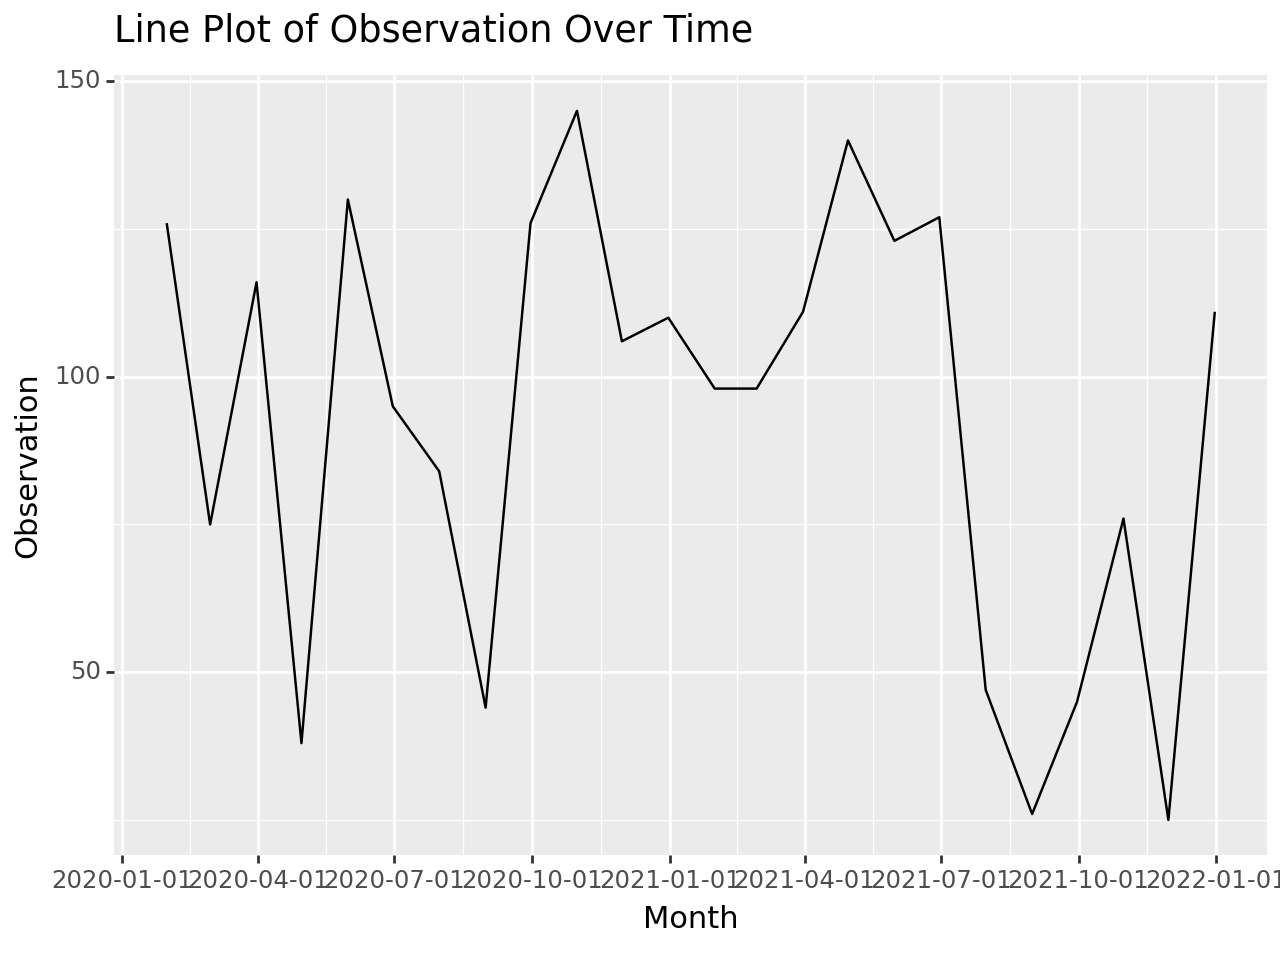
\includegraphics{intro_files/figure-pdf/cell-10-output-1.png}

}

\end{figure}

\begin{verbatim}
\end{verbatim}

\begin{Shaded}
\begin{Highlighting}[]
\NormalTok{plot }\OperatorTok{=}\NormalTok{ (ggplot(monthly\_observation\_df, aes(x}\OperatorTok{=}\StringTok{\textquotesingle{}Month\textquotesingle{}}\NormalTok{, y}\OperatorTok{=}\StringTok{\textquotesingle{}Observation\textquotesingle{}}\NormalTok{)) }\OperatorTok{+}
\NormalTok{        geom\_line() }\OperatorTok{+}
\NormalTok{        geom\_point() }\OperatorTok{+}
\NormalTok{        labs(title}\OperatorTok{=}\StringTok{\textquotesingle{}Line Plot of Observation Over Time\textquotesingle{}}\NormalTok{) }\OperatorTok{+} 
\NormalTok{        scale\_x\_datetime(breaks}\OperatorTok{=}\StringTok{\textquotesingle{}1 month\textquotesingle{}}\NormalTok{,  date\_labels}\OperatorTok{=}\StringTok{\textquotesingle{}\%b \%Y\textquotesingle{}}\NormalTok{) }\OperatorTok{+} 
\NormalTok{        theme(axis\_text\_x}\OperatorTok{=}\NormalTok{element\_text(angle}\OperatorTok{=}\DecValTok{90}\NormalTok{, hjust}\OperatorTok{=}\DecValTok{1}\NormalTok{)))}

\BuiltInTok{print}\NormalTok{(plot)}
\end{Highlighting}
\end{Shaded}

\begin{figure}[H]

{\centering \includegraphics{intro_files/figure-pdf/cell-11-output-1.png}

}

\end{figure}

\begin{verbatim}
\end{verbatim}

\begin{Shaded}
\begin{Highlighting}[]
\NormalTok{plot }\OperatorTok{=}\NormalTok{ (ggplot(monthly\_observation\_df, aes(x}\OperatorTok{=}\StringTok{\textquotesingle{}Month\textquotesingle{}}\NormalTok{, y}\OperatorTok{=}\StringTok{\textquotesingle{}Observation\textquotesingle{}}\NormalTok{)) }\OperatorTok{+}
\NormalTok{        geom\_line() }\OperatorTok{+}
\NormalTok{        geom\_point() }\OperatorTok{+}
\NormalTok{        labs(title}\OperatorTok{=}\StringTok{\textquotesingle{}Line Plot of Observation Over Time\textquotesingle{}}\NormalTok{) }\OperatorTok{+} 
\NormalTok{        scale\_x\_datetime(breaks}\OperatorTok{=}\StringTok{\textquotesingle{}1 month\textquotesingle{}}\NormalTok{,  date\_labels}\OperatorTok{=}\StringTok{\textquotesingle{}\%Y{-}\%m{-}}\SpecialCharTok{\%d}\StringTok{\textquotesingle{}}\NormalTok{) }\OperatorTok{+} 
\NormalTok{        theme(axis\_text\_x}\OperatorTok{=}\NormalTok{element\_text(angle}\OperatorTok{=}\DecValTok{90}\NormalTok{, hjust}\OperatorTok{=}\DecValTok{1}\NormalTok{)))}

\BuiltInTok{print}\NormalTok{(plot)}
\end{Highlighting}
\end{Shaded}

\begin{figure}[H]

{\centering 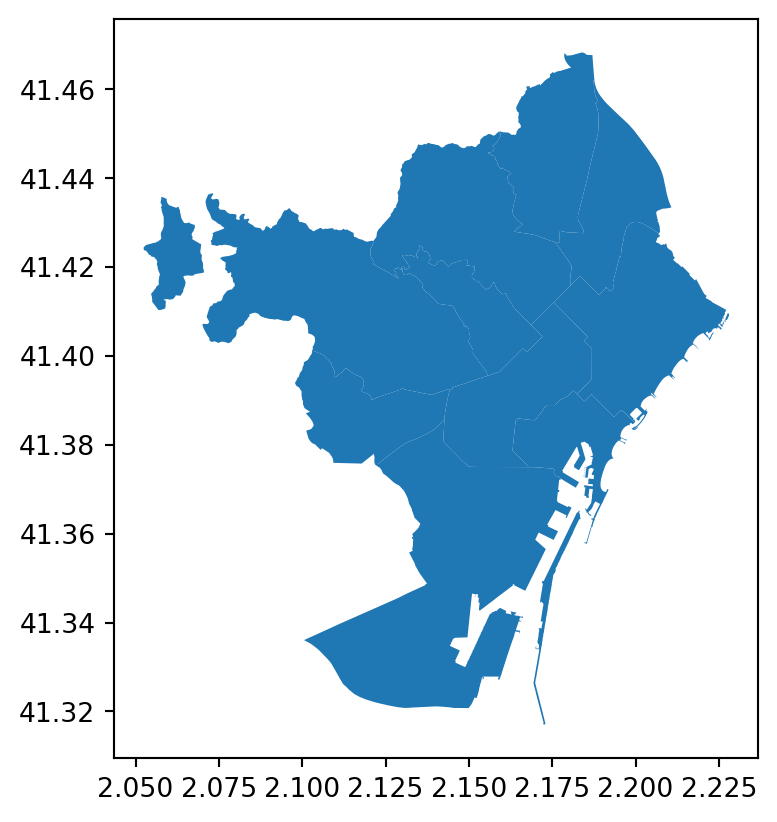
\includegraphics{intro_files/figure-pdf/cell-12-output-1.png}

}

\end{figure}

\begin{verbatim}
\end{verbatim}

\begin{Shaded}
\begin{Highlighting}[]
\NormalTok{plot }\OperatorTok{=}\NormalTok{ (ggplot(monthly\_observation\_df, aes(x}\OperatorTok{=}\StringTok{\textquotesingle{}Month\textquotesingle{}}\NormalTok{, y}\OperatorTok{=}\StringTok{\textquotesingle{}Observation\textquotesingle{}}\NormalTok{)) }\OperatorTok{+}
\NormalTok{        geom\_line() }\OperatorTok{+}
\NormalTok{        geom\_point() }\OperatorTok{+}
\NormalTok{        labs(title}\OperatorTok{=}\StringTok{\textquotesingle{}Line Plot of Observation Over Time\textquotesingle{}}\NormalTok{) }\OperatorTok{+} 
\NormalTok{        scale\_x\_datetime(breaks}\OperatorTok{=}\StringTok{\textquotesingle{}1 month\textquotesingle{}}\NormalTok{,  date\_labels}\OperatorTok{=}\StringTok{\textquotesingle{}\%m \%Y\textquotesingle{}}\NormalTok{) }\OperatorTok{+} 
\NormalTok{        theme(axis\_text\_x}\OperatorTok{=}\NormalTok{element\_text(angle}\OperatorTok{=}\DecValTok{90}\NormalTok{, hjust}\OperatorTok{=}\DecValTok{1}\NormalTok{)))}

\BuiltInTok{print}\NormalTok{(plot)}
\end{Highlighting}
\end{Shaded}

\begin{figure}[H]

{\centering 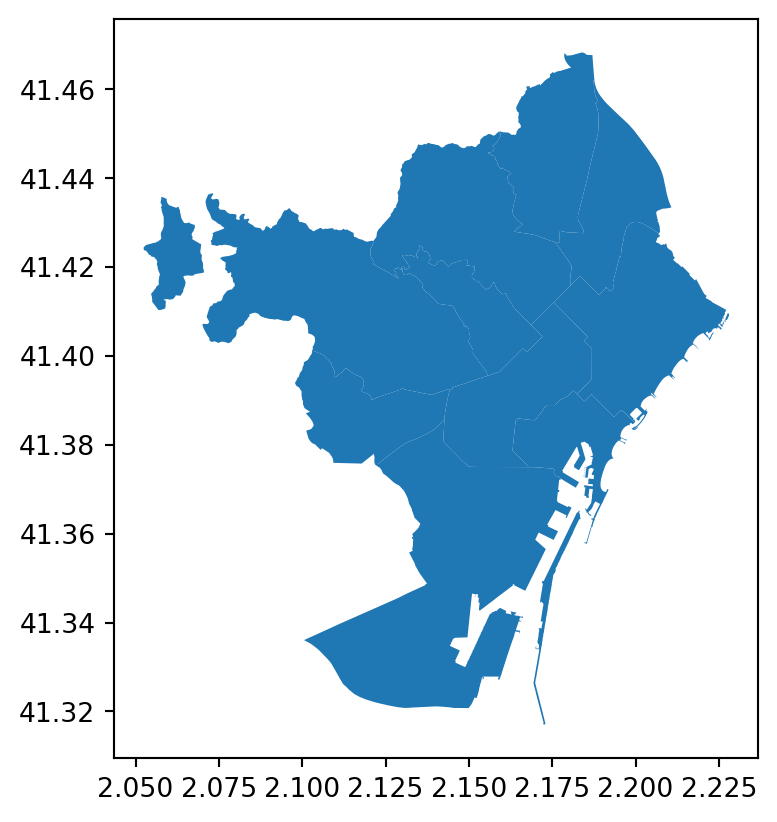
\includegraphics{intro_files/figure-pdf/cell-13-output-1.png}

}

\end{figure}

\begin{verbatim}
\end{verbatim}

\begin{verbatim}
\end{verbatim}

\begin{itemize}
\item
  \textbf{\texttt{\%Y}}: Year with century as a decimal number (e.g.,
  2023).
\item
  \textbf{\texttt{\%m}}: Month as a zero-padded decimal number (e.g., 01
  for January).
\item
  \textbf{\texttt{\%d}}: Day of the month as a zero-padded decimal
  number (e.g., 07).
\end{itemize}

\begin{verbatim}
\end{verbatim}

\begin{Shaded}
\begin{Highlighting}[]
\NormalTok{date\_range }\OperatorTok{=}\NormalTok{ pd.date\_range(start}\OperatorTok{=}\StringTok{\textquotesingle{}2019{-}01{-}01\textquotesingle{}}\NormalTok{, end}\OperatorTok{=}\StringTok{\textquotesingle{}2019{-}05{-}31\textquotesingle{}}\NormalTok{, freq}\OperatorTok{=}\StringTok{\textquotesingle{}M\textquotesingle{}}\NormalTok{)}
\NormalTok{df\_monthly }\OperatorTok{=}\NormalTok{ pd.DataFrame()}
\CommentTok{\# Add the date range as a \textquotesingle{}Month\textquotesingle{} column}
\NormalTok{df\_monthly[}\StringTok{\textquotesingle{}Month\textquotesingle{}}\NormalTok{] }\OperatorTok{=}\NormalTok{ date\_range}
\NormalTok{df\_monthly[}\StringTok{\textquotesingle{}Observation\textquotesingle{}}\NormalTok{] }\OperatorTok{=}\NormalTok{ [}\DecValTok{50}\NormalTok{, }\DecValTok{23}\NormalTok{, }\DecValTok{34}\NormalTok{, }\DecValTok{30}\NormalTok{, }\DecValTok{25}\NormalTok{]}

\CommentTok{\# Display the resulting DataFrame}
\BuiltInTok{print}\NormalTok{(}\StringTok{"Monthly DataFrame:"}\NormalTok{)}
\BuiltInTok{print}\NormalTok{(df\_monthly)}
\NormalTok{df\_monthly.info()}
\NormalTok{plot }\OperatorTok{=}\NormalTok{ (ggplot(df\_monthly, aes(x}\OperatorTok{=}\StringTok{\textquotesingle{}Month\textquotesingle{}}\NormalTok{, y}\OperatorTok{=}\StringTok{\textquotesingle{}Observation\textquotesingle{}}\NormalTok{)) }\OperatorTok{+}
\NormalTok{        geom\_line() }\OperatorTok{+}
\NormalTok{       labs(title}\OperatorTok{=}\StringTok{\textquotesingle{}Line Plot of Observation Over Time\textquotesingle{}}\NormalTok{) }\OperatorTok{+} 
\NormalTok{       scale\_x\_datetime(breaks}\OperatorTok{=}\StringTok{\textquotesingle{}1 month\textquotesingle{}}\NormalTok{))}
\BuiltInTok{print}\NormalTok{(plot)}
\end{Highlighting}
\end{Shaded}

\begin{verbatim}
Monthly DataFrame:
       Month  Observation
0 2019-01-31           50
1 2019-02-28           23
2 2019-03-31           34
3 2019-04-30           30
4 2019-05-31           25
<class 'pandas.core.frame.DataFrame'>
RangeIndex: 5 entries, 0 to 4
Data columns (total 2 columns):
 #   Column       Non-Null Count  Dtype         
---  ------       --------------  -----         
 0   Month        5 non-null      datetime64[ns]
 1   Observation  5 non-null      int64         
dtypes: datetime64[ns](1), int64(1)
memory usage: 212.0 bytes
\end{verbatim}

\begin{figure}[H]

{\centering 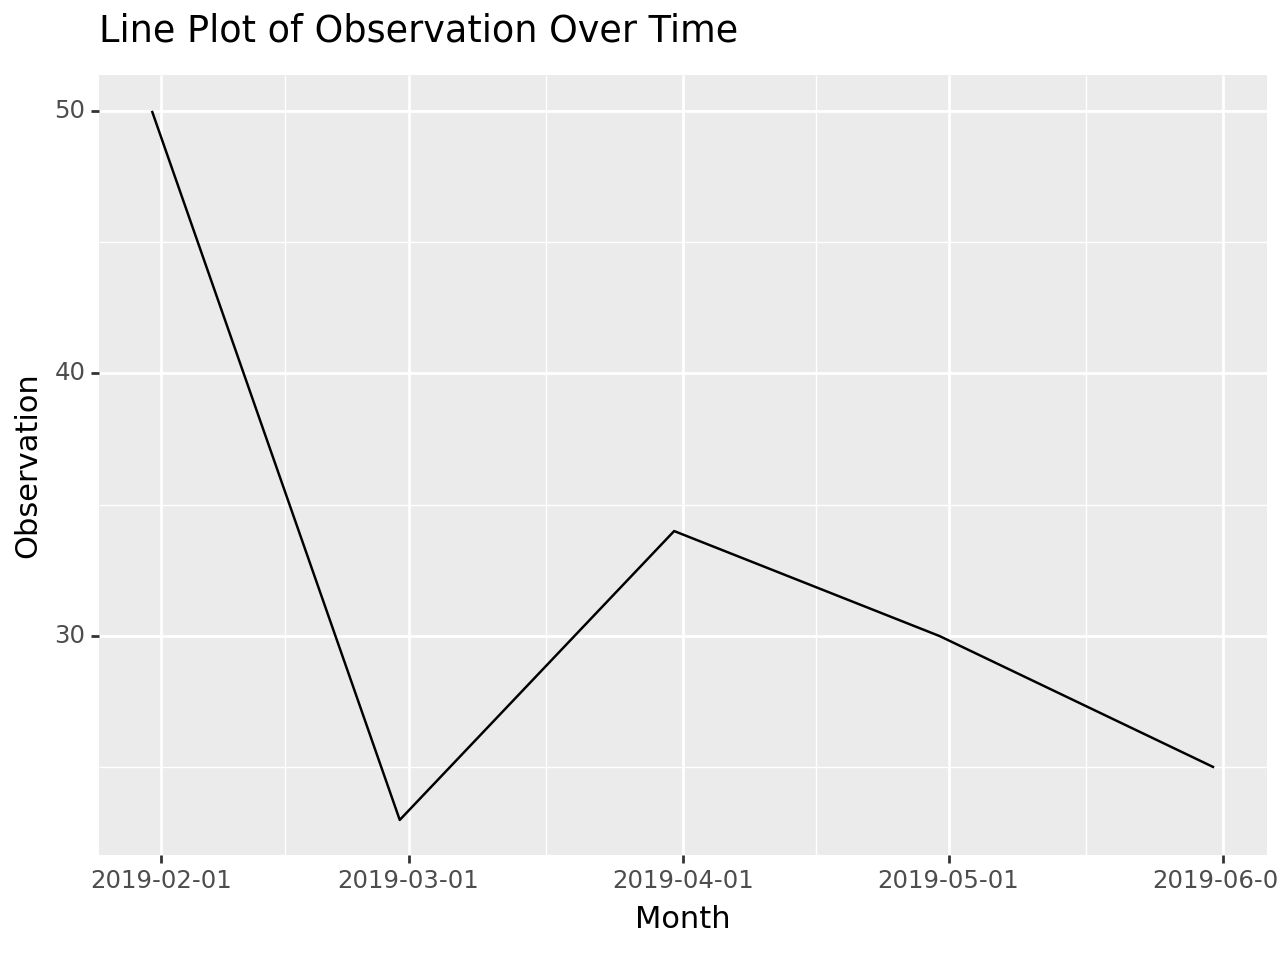
\includegraphics{intro_files/figure-pdf/cell-14-output-2.png}

}

\end{figure}

\begin{verbatim}
\end{verbatim}

\hypertarget{weekly}{%
\subsection{Weekly}\label{weekly}}

\begin{Shaded}
\begin{Highlighting}[]
\NormalTok{start\_date }\OperatorTok{=} \StringTok{\textquotesingle{}2015{-}01{-}01\textquotesingle{}}
\NormalTok{end\_date }\OperatorTok{=} \StringTok{\textquotesingle{}2020{-}12{-}31\textquotesingle{}}

\NormalTok{weekly\_dates }\OperatorTok{=}\NormalTok{ pd.date\_range(start}\OperatorTok{=}\NormalTok{start\_date, end}\OperatorTok{=}\NormalTok{end\_date, freq}\OperatorTok{=}\StringTok{\textquotesingle{}W\textquotesingle{}}\NormalTok{)}
\BuiltInTok{print}\NormalTok{(}\StringTok{"Weekly Dates:"}\NormalTok{)}
\BuiltInTok{print}\NormalTok{(weekly\_dates)}
\end{Highlighting}
\end{Shaded}

\begin{verbatim}
Weekly Dates:
DatetimeIndex(['2015-01-04', '2015-01-11', '2015-01-18', '2015-01-25',
               '2015-02-01', '2015-02-08', '2015-02-15', '2015-02-22',
               '2015-03-01', '2015-03-08',
               ...
               '2020-10-25', '2020-11-01', '2020-11-08', '2020-11-15',
               '2020-11-22', '2020-11-29', '2020-12-06', '2020-12-13',
               '2020-12-20', '2020-12-27'],
              dtype='datetime64[ns]', length=313, freq='W-SUN')
\end{verbatim}

\begin{verbatim}
\end{verbatim}

\hypertarget{hourly}{%
\subsection{Hourly}\label{hourly}}

\begin{Shaded}
\begin{Highlighting}[]
\NormalTok{start\_date }\OperatorTok{=} \StringTok{\textquotesingle{}2015{-}01{-}01 00:00:00\textquotesingle{}}
\NormalTok{end\_date }\OperatorTok{=} \StringTok{\textquotesingle{}2015{-}01{-}01 23:59:59\textquotesingle{}}

\NormalTok{hourly\_dates }\OperatorTok{=}\NormalTok{ pd.date\_range(start}\OperatorTok{=}\NormalTok{start\_date, end}\OperatorTok{=}\NormalTok{end\_date, freq}\OperatorTok{=}\StringTok{\textquotesingle{}H\textquotesingle{}}\NormalTok{)}
\BuiltInTok{print}\NormalTok{(}\StringTok{"Hourly Dates:"}\NormalTok{)}
\BuiltInTok{print}\NormalTok{(hourly\_dates)}
\end{Highlighting}
\end{Shaded}

\begin{verbatim}
Hourly Dates:
DatetimeIndex(['2015-01-01 00:00:00', '2015-01-01 01:00:00',
               '2015-01-01 02:00:00', '2015-01-01 03:00:00',
               '2015-01-01 04:00:00', '2015-01-01 05:00:00',
               '2015-01-01 06:00:00', '2015-01-01 07:00:00',
               '2015-01-01 08:00:00', '2015-01-01 09:00:00',
               '2015-01-01 10:00:00', '2015-01-01 11:00:00',
               '2015-01-01 12:00:00', '2015-01-01 13:00:00',
               '2015-01-01 14:00:00', '2015-01-01 15:00:00',
               '2015-01-01 16:00:00', '2015-01-01 17:00:00',
               '2015-01-01 18:00:00', '2015-01-01 19:00:00',
               '2015-01-01 20:00:00', '2015-01-01 21:00:00',
               '2015-01-01 22:00:00', '2015-01-01 23:00:00'],
              dtype='datetime64[ns]', freq='H')
\end{verbatim}

\texttt{\{\#\#\ Derive\ variables\ from\ the\ time\ column\}}

\begin{verbatim}
\end{verbatim}

\begin{verbatim}
\end{verbatim}

\begin{verbatim}
\end{verbatim}

\begin{Shaded}
\begin{Highlighting}[]

\end{Highlighting}
\end{Shaded}

\begin{verbatim}
\end{verbatim}

\bookmarksetup{startatroot}

\hypertarget{import-data-subsetting-data-based-on-dates-down-sampling-and-upsampling}{%
\chapter{Import data, Subsetting data based on dates, Down sampling and
Upsampling}\label{import-data-subsetting-data-based-on-dates-down-sampling-and-upsampling}}

\begin{Shaded}
\begin{Highlighting}[]
\ImportTok{import}\NormalTok{ pandas }\ImportTok{as}\NormalTok{ pd}
\ImportTok{from}\NormalTok{ pandas }\ImportTok{import} \OperatorTok{*}
\ImportTok{import}\NormalTok{ numpy }\ImportTok{as}\NormalTok{ np}
\ImportTok{import}\NormalTok{ plotnine }\ImportTok{as}\NormalTok{ p9}
\ImportTok{from}\NormalTok{ plotnine }\ImportTok{import} \OperatorTok{*}
\ImportTok{import}\NormalTok{ seaborn }\ImportTok{as}\NormalTok{ sns}
\ImportTok{import}\NormalTok{ matplotlib.pyplot }\ImportTok{as}\NormalTok{ plt}
\ImportTok{import}\NormalTok{ datetime}
\ImportTok{from}\NormalTok{ datetime }\ImportTok{import} \OperatorTok{*}
\end{Highlighting}
\end{Shaded}

\hypertarget{import-csv-with-dates}{%
\section{Import CSV with dates}\label{import-csv-with-dates}}

\begin{Shaded}
\begin{Highlighting}[]
\NormalTok{airpassenger }\OperatorTok{=}\NormalTok{ pd.read\_csv(}\StringTok{\textquotesingle{}data/AirPassengers.csv\textquotesingle{}}\NormalTok{, parse\_dates}\OperatorTok{=}\NormalTok{[}\StringTok{"Month"}\NormalTok{])}
\NormalTok{airpassenger}
\BuiltInTok{print}\NormalTok{(airpassenger.info())}
\end{Highlighting}
\end{Shaded}

\begin{verbatim}
<class 'pandas.core.frame.DataFrame'>
RangeIndex: 144 entries, 0 to 143
Data columns (total 2 columns):
 #   Column       Non-Null Count  Dtype         
---  ------       --------------  -----         
 0   Month        144 non-null    datetime64[ns]
 1   #Passengers  144 non-null    int64         
dtypes: datetime64[ns](1), int64(1)
memory usage: 2.4 KB
None
\end{verbatim}

\begin{Shaded}
\begin{Highlighting}[]
\NormalTok{ggplot(airpassenger, aes(x}\OperatorTok{=}\StringTok{\textquotesingle{}Month\textquotesingle{}}\NormalTok{, y}\OperatorTok{=}\StringTok{\textquotesingle{}\#Passengers\textquotesingle{}}\NormalTok{))}\OperatorTok{+}\NormalTok{geom\_line()}
\end{Highlighting}
\end{Shaded}

\begin{figure}[H]

{\centering 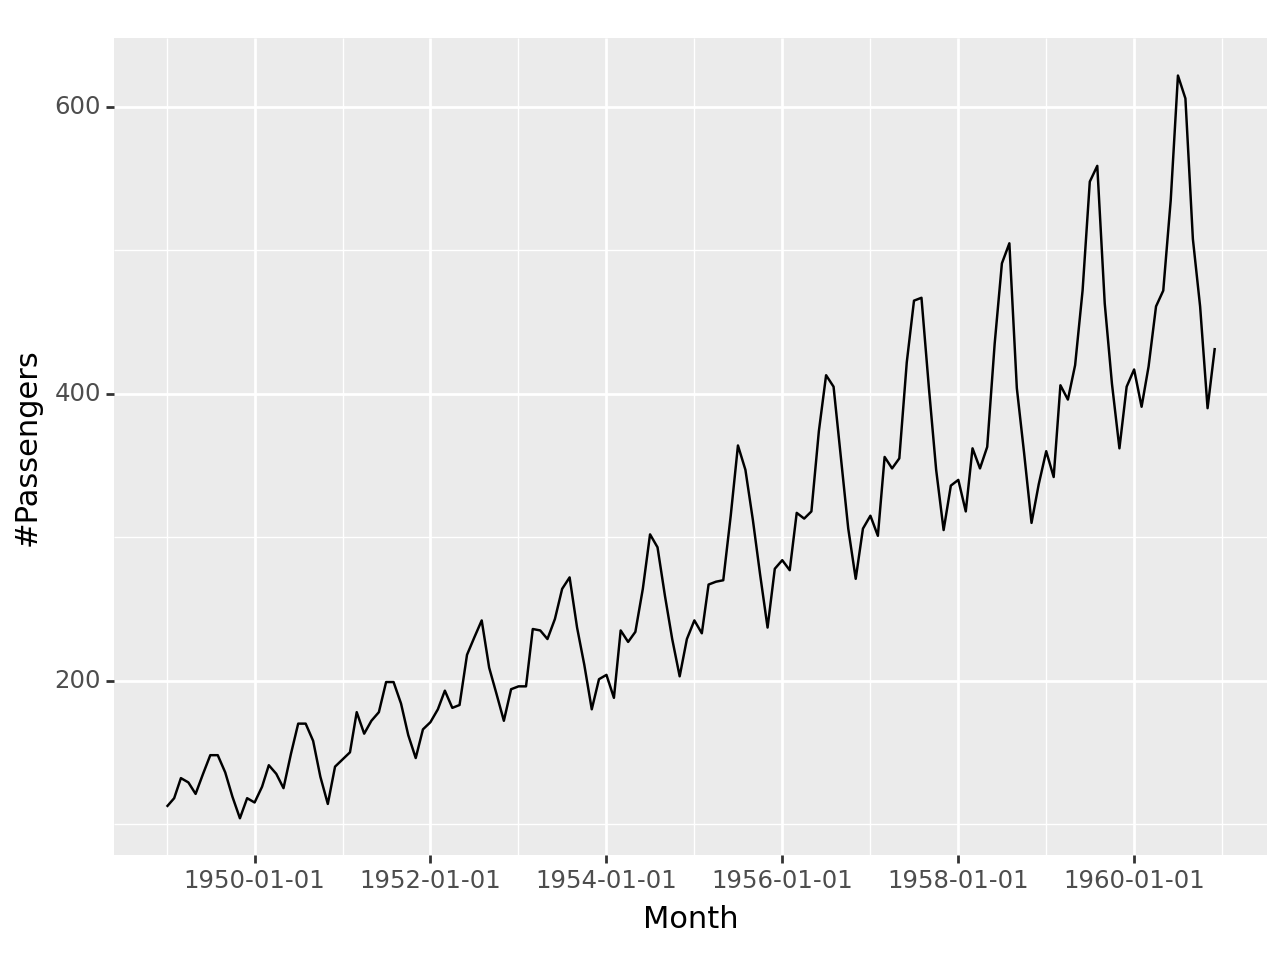
\includegraphics{chap2_files/figure-pdf/cell-4-output-1.png}

}

\end{figure}

\begin{verbatim}
<Figure Size: (640 x 480)>
\end{verbatim}

\begin{Shaded}
\begin{Highlighting}[]
\BuiltInTok{print}\NormalTok{(airpassenger[}\StringTok{\textquotesingle{}Month\textquotesingle{}}\NormalTok{].}\BuiltInTok{min}\NormalTok{())}
\end{Highlighting}
\end{Shaded}

\begin{verbatim}
1949-01-01 00:00:00
\end{verbatim}

\hypertarget{subseting}{%
\section{Subseting}\label{subseting}}

\begin{Shaded}
\begin{Highlighting}[]
\BuiltInTok{print}\NormalTok{(airpassenger.iloc[}\OperatorTok{{-}}\DecValTok{6}\NormalTok{:, :}\DecValTok{6}\NormalTok{])}
\end{Highlighting}
\end{Shaded}

\begin{verbatim}
         Month  #Passengers
138 1960-07-01          622
139 1960-08-01          606
140 1960-09-01          508
141 1960-10-01          461
142 1960-11-01          390
143 1960-12-01          432
\end{verbatim}

\begin{Shaded}
\begin{Highlighting}[]
\BuiltInTok{print}\NormalTok{(airpassenger.iloc[:}\DecValTok{6}\NormalTok{])}
\end{Highlighting}
\end{Shaded}

\begin{verbatim}
       Month  #Passengers
0 1949-01-01          112
1 1949-02-01          118
2 1949-03-01          132
3 1949-04-01          129
4 1949-05-01          121
5 1949-06-01          135
\end{verbatim}

\hypertarget{subsetting-based-on-date-components}{%
\section{Subsetting based on Date
Components}\label{subsetting-based-on-date-components}}

\begin{Shaded}
\begin{Highlighting}[]
\BuiltInTok{print}\NormalTok{(airpassenger.loc[(airpassenger.Month.dt.year }\OperatorTok{==} \DecValTok{1949}\NormalTok{) }\OperatorTok{\&}\NormalTok{ (airpassenger.Month.dt.month }\OperatorTok{==} \DecValTok{8}\NormalTok{)])}
\end{Highlighting}
\end{Shaded}

\begin{verbatim}
       Month  #Passengers
7 1949-08-01          148
\end{verbatim}

\begin{Shaded}
\begin{Highlighting}[]
\BuiltInTok{print}\NormalTok{(airpassenger.loc[(airpassenger.Month.dt.year }\OperatorTok{==} \DecValTok{1949}\NormalTok{) }\OperatorTok{\&}\NormalTok{ (airpassenger.Month.dt.month }\OperatorTok{\textgreater{}} \DecValTok{8}\NormalTok{)])}
\end{Highlighting}
\end{Shaded}

\begin{verbatim}
        Month  #Passengers
8  1949-09-01          136
9  1949-10-01          119
10 1949-11-01          104
11 1949-12-01          118
\end{verbatim}

\begin{Shaded}
\begin{Highlighting}[]
\BuiltInTok{print}\NormalTok{(airpassenger.loc[(airpassenger.Month.dt.year }\OperatorTok{==} \DecValTok{1949}\NormalTok{)])}
\end{Highlighting}
\end{Shaded}

\begin{verbatim}
        Month  #Passengers
0  1949-01-01          112
1  1949-02-01          118
2  1949-03-01          132
3  1949-04-01          129
4  1949-05-01          121
5  1949-06-01          135
6  1949-07-01          148
7  1949-08-01          148
8  1949-09-01          136
9  1949-10-01          119
10 1949-11-01          104
11 1949-12-01          118
\end{verbatim}

\hypertarget{datetimeindex-pandas-time-series-index-by-time}{%
\section{DatetimeIndex: pandas time series index by
time}\label{datetimeindex-pandas-time-series-index-by-time}}

When working with datetime data, it is often required to set the
datetime object to be the index of the dataframe.

\begin{Shaded}
\begin{Highlighting}[]
\NormalTok{airpassenger.index }\OperatorTok{=}\NormalTok{ airpassenger[}\StringTok{\textquotesingle{}Month\textquotesingle{}}\NormalTok{]}
\BuiltInTok{print}\NormalTok{(airpassenger.index)}
\end{Highlighting}
\end{Shaded}

\begin{verbatim}
DatetimeIndex(['1949-01-01', '1949-02-01', '1949-03-01', '1949-04-01',
               '1949-05-01', '1949-06-01', '1949-07-01', '1949-08-01',
               '1949-09-01', '1949-10-01',
               ...
               '1960-03-01', '1960-04-01', '1960-05-01', '1960-06-01',
               '1960-07-01', '1960-08-01', '1960-09-01', '1960-10-01',
               '1960-11-01', '1960-12-01'],
              dtype='datetime64[ns]', name='Month', length=144, freq=None)
\end{verbatim}

\begin{Shaded}
\begin{Highlighting}[]
\NormalTok{airpassenger}
\end{Highlighting}
\end{Shaded}

\begin{longtable}[]{@{}lll@{}}
\toprule\noalign{}
& Month & \#Passengers \\
Month & & \\
\midrule\noalign{}
\endhead
\bottomrule\noalign{}
\endlastfoot
1949-01-01 & 1949-01-01 & 112 \\
1949-02-01 & 1949-02-01 & 118 \\
1949-03-01 & 1949-03-01 & 132 \\
1949-04-01 & 1949-04-01 & 129 \\
1949-05-01 & 1949-05-01 & 121 \\
... & ... & ... \\
1960-08-01 & 1960-08-01 & 606 \\
1960-09-01 & 1960-09-01 & 508 \\
1960-10-01 & 1960-10-01 & 461 \\
1960-11-01 & 1960-11-01 & 390 \\
1960-12-01 & 1960-12-01 & 432 \\
\end{longtable}

Now we can directly subset rows using date components.

\begin{Shaded}
\begin{Highlighting}[]
\BuiltInTok{print}\NormalTok{(airpassenger.loc[}\StringTok{\textquotesingle{}1949\textquotesingle{}}\NormalTok{])}
\end{Highlighting}
\end{Shaded}

\begin{verbatim}
                Month  #Passengers
Month                             
1949-01-01 1949-01-01          112
1949-02-01 1949-02-01          118
1949-03-01 1949-03-01          132
1949-04-01 1949-04-01          129
1949-05-01 1949-05-01          121
1949-06-01 1949-06-01          135
1949-07-01 1949-07-01          148
1949-08-01 1949-08-01          148
1949-09-01 1949-09-01          136
1949-10-01 1949-10-01          119
1949-11-01 1949-11-01          104
1949-12-01 1949-12-01          118
\end{verbatim}

\begin{Shaded}
\begin{Highlighting}[]
\BuiltInTok{print}\NormalTok{(airpassenger.loc[}\StringTok{\textquotesingle{}1949{-}06\textquotesingle{}}\NormalTok{])}
\end{Highlighting}
\end{Shaded}

\begin{verbatim}
                Month  #Passengers
Month                             
1949-06-01 1949-06-01          135
\end{verbatim}

\hypertarget{downsampling}{%
\section{Downsampling}\label{downsampling}}

Downsampling monthly values to yearly values

\begin{Shaded}
\begin{Highlighting}[]
\NormalTok{down }\OperatorTok{=}\NormalTok{ airpassenger.resample(}\StringTok{\textquotesingle{}Y\textquotesingle{}}\NormalTok{).mean()}
\NormalTok{down}
\end{Highlighting}
\end{Shaded}

\begin{longtable}[]{@{}lll@{}}
\toprule\noalign{}
& Month & \#Passengers \\
Month & & \\
\midrule\noalign{}
\endhead
\bottomrule\noalign{}
\endlastfoot
1949-12-31 & 1949-06-16 12:00:00 & 126.666667 \\
1950-12-31 & 1950-06-16 12:00:00 & 139.666667 \\
1951-12-31 & 1951-06-16 12:00:00 & 170.166667 \\
1952-12-31 & 1952-06-16 08:00:00 & 197.000000 \\
1953-12-31 & 1953-06-16 12:00:00 & 225.000000 \\
1954-12-31 & 1954-06-16 12:00:00 & 238.916667 \\
1955-12-31 & 1955-06-16 12:00:00 & 284.000000 \\
1956-12-31 & 1956-06-16 08:00:00 & 328.250000 \\
1957-12-31 & 1957-06-16 12:00:00 & 368.416667 \\
1958-12-31 & 1958-06-16 12:00:00 & 381.000000 \\
1959-12-31 & 1959-06-16 12:00:00 & 428.333333 \\
1960-12-31 & 1960-06-16 08:00:00 & 476.166667 \\
\end{longtable}

\hypertarget{upsampling}{%
\section{Upsampling}\label{upsampling}}

Upsample monthly values to daily values

\begin{Shaded}
\begin{Highlighting}[]
\NormalTok{up }\OperatorTok{=}\NormalTok{ airpassenger.resample(}\StringTok{\textquotesingle{}D\textquotesingle{}}\NormalTok{).mean()}
\NormalTok{up}
\end{Highlighting}
\end{Shaded}

\begin{longtable}[]{@{}lll@{}}
\toprule\noalign{}
& Month & \#Passengers \\
Month & & \\
\midrule\noalign{}
\endhead
\bottomrule\noalign{}
\endlastfoot
1949-01-01 & 1949-01-01 & 112.0 \\
1949-01-02 & NaT & NaN \\
1949-01-03 & NaT & NaN \\
1949-01-04 & NaT & NaN \\
1949-01-05 & NaT & NaN \\
... & ... & ... \\
1960-11-27 & NaT & NaN \\
1960-11-28 & NaT & NaN \\
1960-11-29 & NaT & NaN \\
1960-11-30 & NaT & NaN \\
1960-12-01 & 1960-12-01 & 432.0 \\
\end{longtable}

\bookmarksetup{startatroot}

\hypertarget{time-series-graphics}{%
\chapter{Time Series Graphics}\label{time-series-graphics}}

\begin{Shaded}
\begin{Highlighting}[]
\ImportTok{import}\NormalTok{ pandas }\ImportTok{as}\NormalTok{ pd}
\ImportTok{from}\NormalTok{ pandas }\ImportTok{import} \OperatorTok{*}
\ImportTok{import}\NormalTok{ numpy }\ImportTok{as}\NormalTok{ np}
\ImportTok{import}\NormalTok{ plotnine }\ImportTok{as}\NormalTok{ p9}
\ImportTok{from}\NormalTok{ plotnine }\ImportTok{import} \OperatorTok{*}
\ImportTok{import}\NormalTok{ seaborn }\ImportTok{as}\NormalTok{ sns}
\ImportTok{import}\NormalTok{ matplotlib.pyplot }\ImportTok{as}\NormalTok{ plt}
\ImportTok{import}\NormalTok{ datetime}
\ImportTok{from}\NormalTok{ datetime }\ImportTok{import} \OperatorTok{*}
\end{Highlighting}
\end{Shaded}

\hypertarget{task-1}{%
\section{Task 1}\label{task-1}}

\begin{enumerate}
\def\labelenumi{\arabic{enumi}.}
\tightlist
\item
  Get data from tsibbledata package in R and write it as a csv file
\end{enumerate}

Following is an R code.

\begin{Shaded}
\begin{Highlighting}[]
\CommentTok{\#install.packages("tsibbledata")}
\FunctionTok{library}\NormalTok{(tsibbledata)}
\FunctionTok{library}\NormalTok{(tidyverse)}
\FunctionTok{data}\NormalTok{(olympic\_running)}
\FunctionTok{write\_csv}\NormalTok{(olympic\_running, }\AttributeTok{file=}\StringTok{"data/olympic\_running.csv"}\NormalTok{)}
\end{Highlighting}
\end{Shaded}

\begin{enumerate}
\def\labelenumi{\arabic{enumi}.}
\setcounter{enumi}{1}
\tightlist
\item
  Read data
\end{enumerate}

\begin{Shaded}
\begin{Highlighting}[]
\NormalTok{olympic\_running }\OperatorTok{=}\NormalTok{ pd.read\_csv(}\StringTok{\textquotesingle{}data/olympic\_running.csv\textquotesingle{}}\NormalTok{, parse\_dates}\OperatorTok{=}\NormalTok{[}\StringTok{\textquotesingle{}Year\textquotesingle{}}\NormalTok{])}
\NormalTok{olympic\_running}
\end{Highlighting}
\end{Shaded}

\begin{longtable}[]{@{}lllll@{}}
\toprule\noalign{}
& Year & Length & Sex & Time \\
\midrule\noalign{}
\endhead
\bottomrule\noalign{}
\endlastfoot
0 & 1896-01-01 & 100 & men & 12.00 \\
1 & 1900-01-01 & 100 & men & 11.00 \\
2 & 1904-01-01 & 100 & men & 11.00 \\
3 & 1908-01-01 & 100 & men & 10.80 \\
4 & 1912-01-01 & 100 & men & 10.80 \\
... & ... & ... & ... & ... \\
307 & 2000-01-01 & 10000 & women & 1817.49 \\
308 & 2004-01-01 & 10000 & women & 1824.36 \\
309 & 2008-01-01 & 10000 & women & 1794.66 \\
310 & 2012-01-01 & 10000 & women & 1820.75 \\
311 & 2016-01-01 & 10000 & women & 1757.45 \\
\end{longtable}

Task: Visualise data in a meaningful way.

\hypertarget{task-2}{%
\section{Task 2}\label{task-2}}

Obtain \texttt{vic\_elec} data from the \texttt{tsibbledata} package in
R and visualize.

Help

\begin{Shaded}
\begin{Highlighting}[]
\ImportTok{import}\NormalTok{ pandas }\ImportTok{as}\NormalTok{ pd}
\NormalTok{vic\_elec }\OperatorTok{=}\NormalTok{ pd.read\_csv(}\StringTok{\textquotesingle{}data/vic\_elec.csv\textquotesingle{}}\NormalTok{, parse\_dates}\OperatorTok{=}\NormalTok{[}\StringTok{\textquotesingle{}Time\textquotesingle{}}\NormalTok{])}
\NormalTok{vic\_elec}
\end{Highlighting}
\end{Shaded}

\begin{longtable}[]{@{}llllll@{}}
\toprule\noalign{}
& Time & Demand & Temperature & Date & Holiday \\
\midrule\noalign{}
\endhead
\bottomrule\noalign{}
\endlastfoot
0 & 2011-12-31 13:00:00+00:00 & 4382.825174 & 21.40 & 2012-01-01 &
True \\
1 & 2011-12-31 13:30:00+00:00 & 4263.365526 & 21.05 & 2012-01-01 &
True \\
2 & 2011-12-31 14:00:00+00:00 & 4048.966046 & 20.70 & 2012-01-01 &
True \\
3 & 2011-12-31 14:30:00+00:00 & 3877.563330 & 20.55 & 2012-01-01 &
True \\
4 & 2011-12-31 15:00:00+00:00 & 4036.229746 & 20.40 & 2012-01-01 &
True \\
... & ... & ... & ... & ... & ... \\
52603 & 2014-12-31 10:30:00+00:00 & 3873.448714 & 19.00 & 2014-12-31 &
False \\
52604 & 2014-12-31 11:00:00+00:00 & 3791.637322 & 18.50 & 2014-12-31 &
False \\
52605 & 2014-12-31 11:30:00+00:00 & 3724.835666 & 17.70 & 2014-12-31 &
False \\
52606 & 2014-12-31 12:00:00+00:00 & 3761.886854 & 17.30 & 2014-12-31 &
False \\
52607 & 2014-12-31 12:30:00+00:00 & 3809.414586 & 17.10 & 2014-12-31 &
False \\
\end{longtable}

\begin{Shaded}
\begin{Highlighting}[]
\NormalTok{vic\_elec.info()}
\end{Highlighting}
\end{Shaded}

\begin{verbatim}
<class 'pandas.core.frame.DataFrame'>
RangeIndex: 52608 entries, 0 to 52607
Data columns (total 5 columns):
 #   Column       Non-Null Count  Dtype              
---  ------       --------------  -----              
 0   Time         52608 non-null  datetime64[ns, UTC]
 1   Demand       52608 non-null  float64            
 2   Temperature  52608 non-null  float64            
 3   Date         52608 non-null  object             
 4   Holiday      52608 non-null  bool               
dtypes: bool(1), datetime64[ns, UTC](1), float64(2), object(1)
memory usage: 1.7+ MB
\end{verbatim}

\bookmarksetup{startatroot}

\hypertarget{time-series-decomposition}{%
\chapter{Time Series Decomposition}\label{time-series-decomposition}}

\begin{Shaded}
\begin{Highlighting}[]
\ImportTok{import}\NormalTok{ numpy }\ImportTok{as}\NormalTok{ np}
\ImportTok{import}\NormalTok{ pandas }\ImportTok{as}\NormalTok{ pd}
\ImportTok{import}\NormalTok{ matplotlib.pyplot }\ImportTok{as}\NormalTok{ plt}
\ImportTok{from}\NormalTok{ statsmodels.tsa.seasonal }\ImportTok{import}\NormalTok{ STL}

\CommentTok{\# Load the AirPassengers dataset}
\NormalTok{air\_passengers }\OperatorTok{=}\NormalTok{ pd.read\_csv(}\StringTok{\textquotesingle{}data/AirPassengers.csv\textquotesingle{}}\NormalTok{)}
\NormalTok{air\_passengers[}\StringTok{\textquotesingle{}Month\textquotesingle{}}\NormalTok{] }\OperatorTok{=}\NormalTok{ pd.to\_datetime(air\_passengers[}\StringTok{\textquotesingle{}Month\textquotesingle{}}\NormalTok{])}
\NormalTok{air\_passengers.set\_index(}\StringTok{\textquotesingle{}Month\textquotesingle{}}\NormalTok{, inplace}\OperatorTok{=}\VariableTok{True}\NormalTok{)}

\CommentTok{\# Perform STL decomposition}
\NormalTok{stl }\OperatorTok{=}\NormalTok{ STL(air\_passengers, seasonal}\OperatorTok{=}\DecValTok{13}\NormalTok{)  }\CommentTok{\# The seasonal parameter is chosen based on the periodicity of your data}
\NormalTok{result }\OperatorTok{=}\NormalTok{ stl.fit()}
\NormalTok{result}
\end{Highlighting}
\end{Shaded}

\begin{verbatim}
<statsmodels.tsa.seasonal.DecomposeResult at 0x1f07f30b7d0>
\end{verbatim}

\hypertarget{method-1-plotting}{%
\section{Method 1: Plotting}\label{method-1-plotting}}

\begin{Shaded}
\begin{Highlighting}[]
\CommentTok{\# Plot the original time series, trend, seasonal, and remainder components}
\NormalTok{fig, (ax1, ax2, ax3, ax4) }\OperatorTok{=}\NormalTok{ plt.subplots(}\DecValTok{4}\NormalTok{, }\DecValTok{1}\NormalTok{, figsize}\OperatorTok{=}\NormalTok{(}\DecValTok{10}\NormalTok{, }\DecValTok{8}\NormalTok{), sharex}\OperatorTok{=}\VariableTok{True}\NormalTok{)}

\NormalTok{ax1.plot(air\_passengers, label}\OperatorTok{=}\StringTok{\textquotesingle{}Original\textquotesingle{}}\NormalTok{)}
\NormalTok{ax1.legend()}

\NormalTok{ax2.plot(result.trend, label}\OperatorTok{=}\StringTok{\textquotesingle{}Trend\textquotesingle{}}\NormalTok{, color}\OperatorTok{=}\StringTok{\textquotesingle{}orange\textquotesingle{}}\NormalTok{)}
\NormalTok{ax2.legend()}

\NormalTok{ax3.plot(result.seasonal, label}\OperatorTok{=}\StringTok{\textquotesingle{}Seasonal\textquotesingle{}}\NormalTok{, color}\OperatorTok{=}\StringTok{\textquotesingle{}green\textquotesingle{}}\NormalTok{)}
\NormalTok{ax3.legend()}

\NormalTok{ax4.plot(result.resid, label}\OperatorTok{=}\StringTok{\textquotesingle{}Residual\textquotesingle{}}\NormalTok{, color}\OperatorTok{=}\StringTok{\textquotesingle{}red\textquotesingle{}}\NormalTok{)}
\NormalTok{ax4.legend()}

\NormalTok{plt.suptitle(}\StringTok{\textquotesingle{}STL Decomposition of AirPassengers Dataset\textquotesingle{}}\NormalTok{)}
\NormalTok{plt.show()}
\end{Highlighting}
\end{Shaded}

\begin{figure}[H]

{\centering 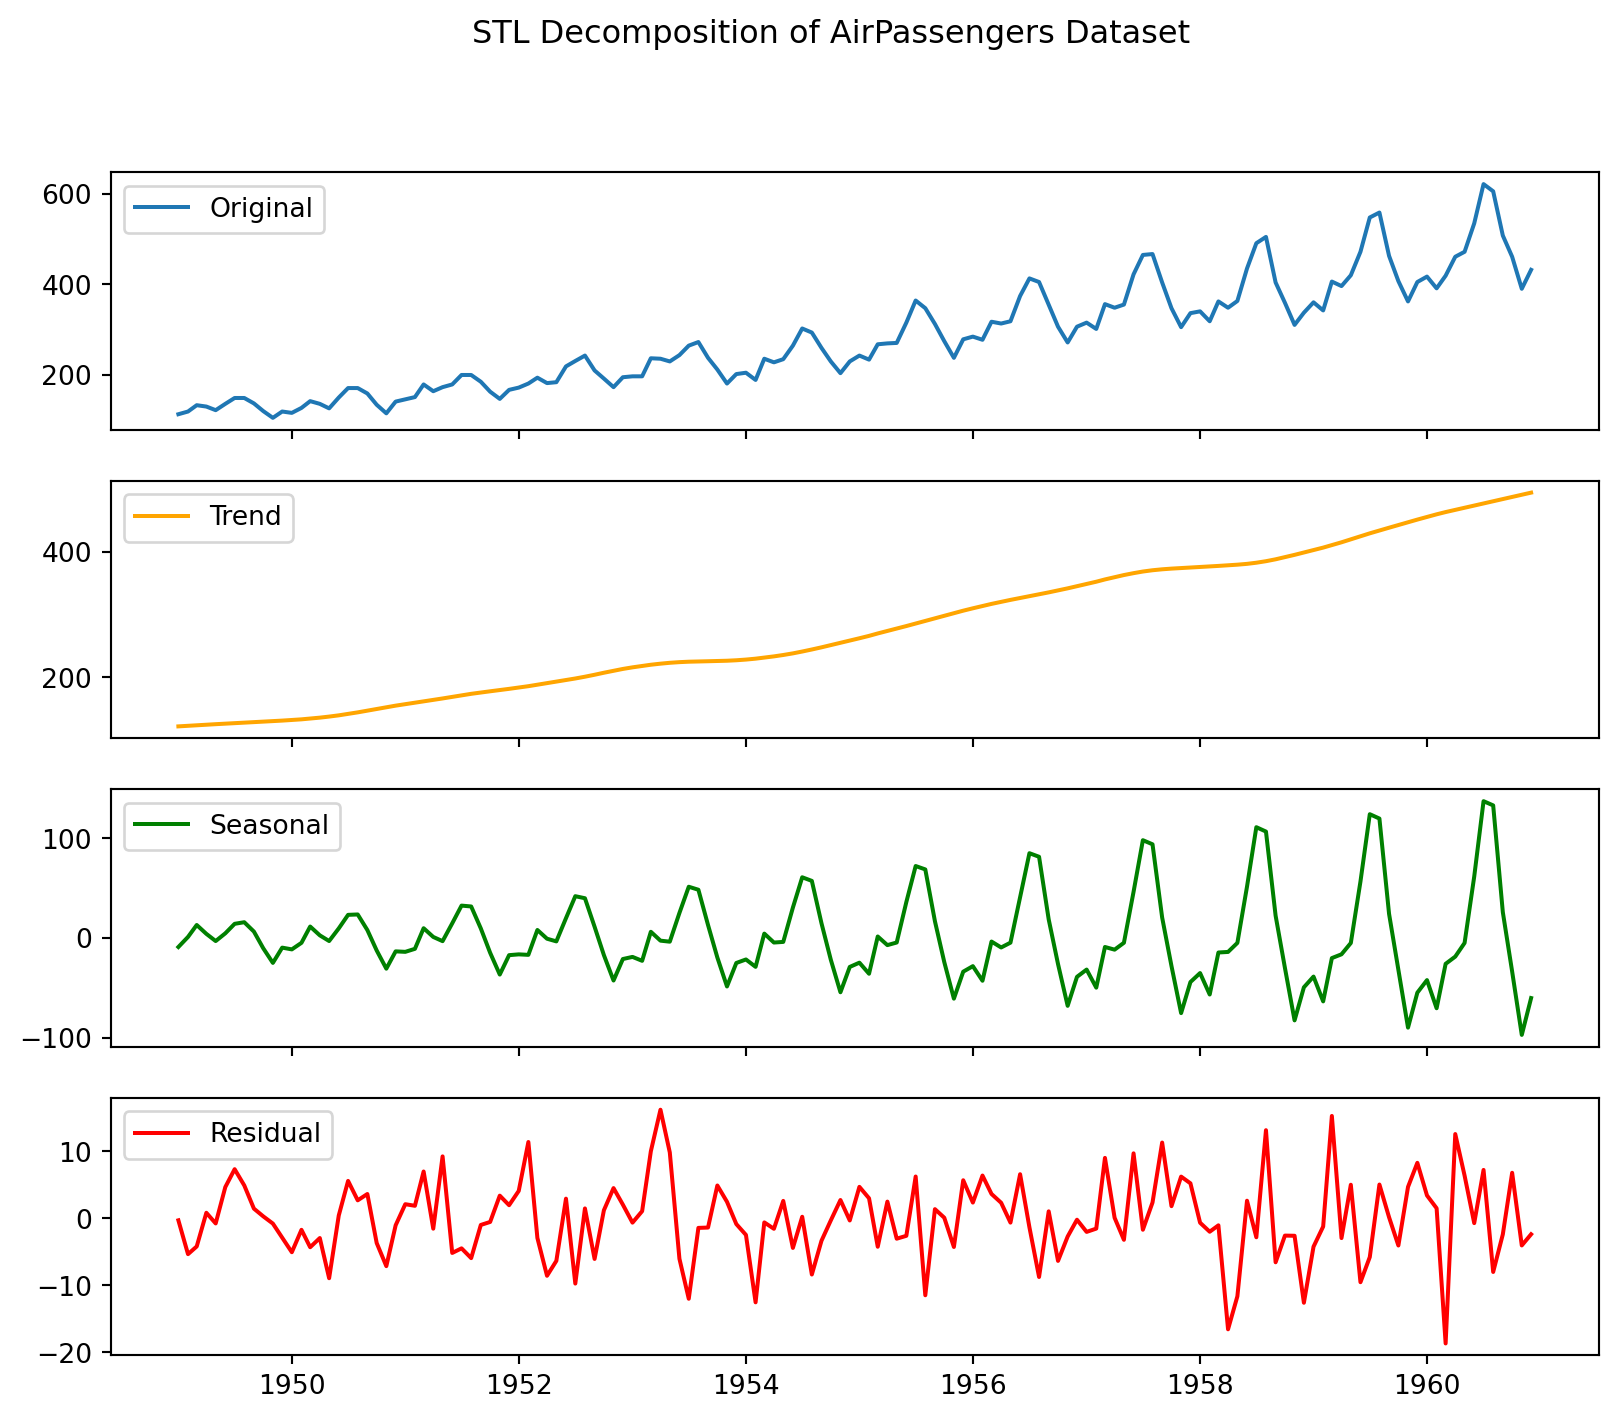
\includegraphics{chap4_files/figure-pdf/cell-3-output-1.pdf}

}

\end{figure}

\hypertarget{method-2-plotting-using-plotnine}{%
\section{Method 2: Plotting using
plotnine}\label{method-2-plotting-using-plotnine}}

\begin{Shaded}
\begin{Highlighting}[]
\ImportTok{from}\NormalTok{ plotnine }\ImportTok{import}\NormalTok{ ggplot, aes, geom\_line, facet\_wrap, ggtitle}
\CommentTok{\# Create a DataFrame for visualization}
\NormalTok{df\_visualization }\OperatorTok{=}\NormalTok{ pd.DataFrame(\{}
    \StringTok{\textquotesingle{}Date\textquotesingle{}}\NormalTok{: air\_passengers.index,}
    \StringTok{\textquotesingle{}Original\textquotesingle{}}\NormalTok{: air\_passengers[}\StringTok{\textquotesingle{}\#Passengers\textquotesingle{}}\NormalTok{],}
    \StringTok{\textquotesingle{}Trend\textquotesingle{}}\NormalTok{: result.trend,}
    \StringTok{\textquotesingle{}Seasonal\textquotesingle{}}\NormalTok{: result.seasonal,}
    \StringTok{\textquotesingle{}Residual\textquotesingle{}}\NormalTok{: result.resid}
\NormalTok{\})}
\NormalTok{df\_visualization}
\end{Highlighting}
\end{Shaded}

\begin{longtable}[]{@{}llllll@{}}
\toprule\noalign{}
& Date & Original & Trend & Seasonal & Residual \\
Month & & & & & \\
\midrule\noalign{}
\endhead
\bottomrule\noalign{}
\endlastfoot
1949-01-01 & 1949-01-01 & 112 & 121.463327 & -9.157113 & -0.306215 \\
1949-02-01 & 1949-02-01 & 118 & 122.392507 & 0.961357 & -5.353864 \\
1949-03-01 & 1949-03-01 & 132 & 123.284151 & 12.919571 & -4.203722 \\
1949-04-01 & 1949-04-01 & 129 & 124.139983 & 4.042554 & 0.817463 \\
1949-05-01 & 1949-05-01 & 121 & 124.967180 & -3.196646 & -0.770534 \\
... & ... & ... & ... & ... & ... \\
1960-08-01 & 1960-08-01 & 606 & 481.142084 & 132.866128 & -8.008212 \\
1960-09-01 & 1960-09-01 & 508 & 484.574794 & 25.826563 & -2.401357 \\
1960-10-01 & 1960-10-01 & 461 & 487.984483 & -33.766745 & 6.782262 \\
1960-11-01 & 1960-11-01 & 390 & 491.372961 & -97.319814 & -4.053148 \\
1960-12-01 & 1960-12-01 & 432 & 494.738728 & -60.351183 & -2.387545 \\
\end{longtable}

\begin{Shaded}
\begin{Highlighting}[]
\CommentTok{\# Melt the DataFrame for easier plotting}
\NormalTok{df\_melted }\OperatorTok{=}\NormalTok{ df\_visualization.melt(id\_vars}\OperatorTok{=}\StringTok{\textquotesingle{}Date\textquotesingle{}}\NormalTok{, var\_name}\OperatorTok{=}\StringTok{\textquotesingle{}Component\textquotesingle{}}\NormalTok{, value\_name}\OperatorTok{=}\StringTok{\textquotesingle{}Value\textquotesingle{}}\NormalTok{)}
\NormalTok{df\_melted}
\end{Highlighting}
\end{Shaded}

\begin{longtable}[]{@{}llll@{}}
\toprule\noalign{}
& Date & Component & Value \\
\midrule\noalign{}
\endhead
\bottomrule\noalign{}
\endlastfoot
0 & 1949-01-01 & Original & 112.000000 \\
1 & 1949-02-01 & Original & 118.000000 \\
2 & 1949-03-01 & Original & 132.000000 \\
3 & 1949-04-01 & Original & 129.000000 \\
4 & 1949-05-01 & Original & 121.000000 \\
... & ... & ... & ... \\
571 & 1960-08-01 & Residual & -8.008212 \\
572 & 1960-09-01 & Residual & -2.401357 \\
573 & 1960-10-01 & Residual & 6.782262 \\
574 & 1960-11-01 & Residual & -4.053148 \\
575 & 1960-12-01 & Residual & -2.387545 \\
\end{longtable}

\begin{Shaded}
\begin{Highlighting}[]
\CommentTok{\# Plot using plotnine}
\NormalTok{plot }\OperatorTok{=}\NormalTok{ (}
\NormalTok{    ggplot(df\_melted, aes(x}\OperatorTok{=}\StringTok{\textquotesingle{}Date\textquotesingle{}}\NormalTok{, y}\OperatorTok{=}\StringTok{\textquotesingle{}Value\textquotesingle{}}\NormalTok{, color}\OperatorTok{=}\StringTok{\textquotesingle{}Component\textquotesingle{}}\NormalTok{)) }\OperatorTok{+}
\NormalTok{    geom\_line() }\OperatorTok{+}
\NormalTok{    facet\_wrap(}\StringTok{\textquotesingle{}\textasciitilde{}Component\textquotesingle{}}\NormalTok{, scales}\OperatorTok{=}\StringTok{\textquotesingle{}free\_y\textquotesingle{}}\NormalTok{) }\OperatorTok{+}
\NormalTok{    ggtitle(}\StringTok{\textquotesingle{}STL Decomposition of AirPassengers Dataset\textquotesingle{}}\NormalTok{)}
\NormalTok{)}

\CommentTok{\# Display the plot}
\BuiltInTok{print}\NormalTok{(plot)}
\end{Highlighting}
\end{Shaded}

\begin{figure}[H]

{\centering \includegraphics{chap4_files/figure-pdf/cell-6-output-1.png}

}

\end{figure}

\begin{verbatim}
\end{verbatim}

\begin{Shaded}
\begin{Highlighting}[]
\CommentTok{\# Plot using plotnine}
\NormalTok{plot }\OperatorTok{=}\NormalTok{ (}
\NormalTok{    ggplot(df\_melted, aes(x}\OperatorTok{=}\StringTok{\textquotesingle{}Date\textquotesingle{}}\NormalTok{, y}\OperatorTok{=}\StringTok{\textquotesingle{}Value\textquotesingle{}}\NormalTok{, color}\OperatorTok{=}\StringTok{\textquotesingle{}Component\textquotesingle{}}\NormalTok{)) }\OperatorTok{+}
\NormalTok{    geom\_line() }\OperatorTok{+}
\NormalTok{    facet\_wrap(}\StringTok{\textquotesingle{}\textasciitilde{}Component\textquotesingle{}}\NormalTok{, scales}\OperatorTok{=}\StringTok{\textquotesingle{}free\_y\textquotesingle{}}\NormalTok{, ncol}\OperatorTok{=}\DecValTok{1}\NormalTok{) }\OperatorTok{+}
\NormalTok{    ggtitle(}\StringTok{\textquotesingle{}STL Decomposition of AirPassengers Dataset\textquotesingle{}}\NormalTok{)}
\NormalTok{)}

\CommentTok{\# Display the plot}
\BuiltInTok{print}\NormalTok{(plot)}
\end{Highlighting}
\end{Shaded}

\begin{figure}[H]

{\centering \includegraphics{chap4_files/figure-pdf/cell-7-output-1.png}

}

\end{figure}

\begin{verbatim}
\end{verbatim}

Task: Take hourly series and perform STL decomposition.

\bookmarksetup{startatroot}

\hypertarget{time-series-forecasting}{%
\chapter{Time Series Forecasting}\label{time-series-forecasting}}

Please go to course web.

\bookmarksetup{startatroot}

\hypertarget{time-series-features}{%
\chapter{Time Series Features}\label{time-series-features}}

Please go to the course web.

\bookmarksetup{startatroot}

\hypertarget{spatial-visualization}{%
\chapter{Spatial Visualization}\label{spatial-visualization}}

\begin{Shaded}
\begin{Highlighting}[]
\ImportTok{import}\NormalTok{ geopandas }\ImportTok{as}\NormalTok{ gpd}
\ImportTok{import}\NormalTok{ geodatasets}
\end{Highlighting}
\end{Shaded}

\hypertarget{vector-files}{%
\section{Vector files}\label{vector-files}}

\begin{enumerate}
\def\labelenumi{\arabic{enumi}.}
\tightlist
\item
  Shapefiles
\end{enumerate}

\begin{itemize}
\item
  .shp file contains shape geometry
\item
  .dbf file holds attributes for each geometry
\item
  .shx file or shape index file helps link the attributes to the shapes
\end{itemize}

\begin{enumerate}
\def\labelenumi{\arabic{enumi}.}
\setcounter{enumi}{1}
\tightlist
\item
  GeoJSON: Unlike shapefiles, GeoJSON is a single file
\end{enumerate}

\begin{Shaded}
\begin{Highlighting}[]
\NormalTok{chicago }\OperatorTok{=}\NormalTok{ gpd.read\_file(geodatasets.get\_path(}\StringTok{"geoda.chicago\_commpop"}\NormalTok{))}
\NormalTok{chicago}
\NormalTok{chicago.crs}
\end{Highlighting}
\end{Shaded}

\begin{verbatim}
<Geographic 2D CRS: EPSG:4326>
Name: WGS 84
Axis Info [ellipsoidal]:
- Lat[north]: Geodetic latitude (degree)
- Lon[east]: Geodetic longitude (degree)
Area of Use:
- name: World.
- bounds: (-180.0, -90.0, 180.0, 90.0)
Datum: World Geodetic System 1984 ensemble
- Ellipsoid: WGS 84
- Prime Meridian: Greenwich
\end{verbatim}

\begin{Shaded}
\begin{Highlighting}[]
\NormalTok{groceries }\OperatorTok{=}\NormalTok{ gpd.read\_file(geodatasets.get\_path(}\StringTok{"geoda.groceries"}\NormalTok{))}
\NormalTok{groceries}
\end{Highlighting}
\end{Shaded}

\begin{longtable}[]{@{}lllllllll@{}}
\toprule\noalign{}
& OBJECTID & Ycoord & Xcoord & Status & Address & Chain & Category &
geometry \\
\midrule\noalign{}
\endhead
\bottomrule\noalign{}
\endlastfoot
0 & 16 & 41.973266 & -87.657073 & OPEN & 1051 W ARGYLE ST, CHICAGO, IL.
60640 & VIET HOA PLAZA & None & MULTIPOINT (1168268.672 1933554.350) \\
1 & 18 & 41.696367 & -87.681315 & OPEN & 10800 S WESTERN AVE, CHICAGO,
IL. 60643-3226 & COUNTY FAIR FOODS & None & MULTIPOINT (1162302.618
1832900.224) \\
2 & 22 & 41.868634 & -87.638638 & OPEN & 1101 S CANAL ST, CHICAGO, IL.
60607-4932 & WHOLE FOODS MARKET & None & MULTIPOINT (1173317.042
1895425.426) \\
3 & 23 & 41.877590 & -87.654953 & OPEN & 1101 W JACKSON BLVD, CHICAGO,
IL. 60607-2905 & TARGET/SUPER & new & MULTIPOINT (1168996.475
1898801.406) \\
4 & 27 & 41.737696 & -87.625795 & OPEN & 112 W 87TH ST, CHICAGO, IL.
60620-1318 & FOOD 4 LESS & None & MULTIPOINT (1176991.989
1847262.423) \\
... & ... & ... & ... & ... & ... & ... & ... & ... \\
143 & 585 & 41.880834 & -87.647729 & Chicago-West Loop & 40 S Halsted
St, Chicago, IL 60661 & Mariano\textquotesingle s & None & MULTIPOINT
(1171065.063 1899839.376) \\
144 & 586 & 41.920842 & -87.669112 & NewLocation & 2112 N Ashland Ave,
Chicago IL 60614 & Mariano\textquotesingle s & None & MULTIPOINT
(1165217.798 1914159.975) \\
145 & 587 & 41.835930 & -87.664034 & Chicago-Bridgeport & 3145 S Ashland
Ave, Chicago, IL 60608 & Mariano\textquotesingle s & None & MULTIPOINT
(1166186.713 1883581.309) \\
146 & 588 & 41.859370 & -87.630062 & Chicago-South Loop & 1615 S Clark
St, Chicago, IL 60616 & Mariano\textquotesingle s & None & MULTIPOINT
(1175778.816 1892214.445) \\
147 & 600 & 41.696869 & -87.599163 & New Location & 10900 S Doty Ave,
Chicago IL 60628 & Pullman Walmart Center & None & MULTIPOINT
(1185013.734 1832012.356) \\
\end{longtable}

\begin{Shaded}
\begin{Highlighting}[]
\NormalTok{chicago.plot()}\OperatorTok{;}
\end{Highlighting}
\end{Shaded}

\begin{figure}[H]

{\centering \includegraphics{chap7_files/figure-pdf/cell-5-output-1.pdf}

}

\end{figure}

\begin{Shaded}
\begin{Highlighting}[]
\NormalTok{chicago.plot(column}\OperatorTok{=}\StringTok{"POP2010"}\NormalTok{, legend}\OperatorTok{=}\VariableTok{True}\NormalTok{)}\OperatorTok{;}
\end{Highlighting}
\end{Shaded}

\begin{figure}[H]

{\centering \includegraphics{chap7_files/figure-pdf/cell-6-output-1.pdf}

}

\end{figure}

\begin{Shaded}
\begin{Highlighting}[]
\NormalTok{chicago.boundary.plot()}\OperatorTok{;}
\end{Highlighting}
\end{Shaded}

\begin{figure}[H]

{\centering \includegraphics{chap7_files/figure-pdf/cell-7-output-1.pdf}

}

\end{figure}

\hypertarget{centroid}{%
\section{Centroid}\label{centroid}}

Centroid: center point of a geometry.

\begin{Shaded}
\begin{Highlighting}[]
\NormalTok{chicago[}\StringTok{\textquotesingle{}centroid\textquotesingle{}}\NormalTok{]}\OperatorTok{=}\NormalTok{chicago.centroid}
\NormalTok{chicago}
\end{Highlighting}
\end{Shaded}

\begin{verbatim}
C:\Users\DELL\AppData\Local\Temp\ipykernel_29656\3913322276.py:1: UserWarning: Geometry is in a geographic CRS. Results from 'centroid' are likely incorrect. Use 'GeoSeries.to_crs()' to re-project geometries to a projected CRS before this operation.

  chicago['centroid']=chicago.centroid
\end{verbatim}

\begin{longtable}[]{@{}lllllllllll@{}}
\toprule\noalign{}
& community & NID & POP2010 & POP2000 & POPCH & POPPERCH & popplus &
popneg & geometry & centroid \\
\midrule\noalign{}
\endhead
\bottomrule\noalign{}
\endlastfoot
0 & DOUGLAS & 35 & 18238 & 26470 & -8232 & -31.099358 & 0 & 1 &
MULTIPOLYGON (((-87.60914 41.84469, -87.60915 ... & POINT (-87.61868
41.83512) \\
1 & OAKLAND & 36 & 5918 & 6110 & -192 & -3.142390 & 0 & 1 & MULTIPOLYGON
(((-87.59215 41.81693, -87.59231 ... & POINT (-87.60322 41.82375) \\
2 & FULLER PARK & 37 & 2876 & 3420 & -544 & -15.906433 & 0 & 1 &
MULTIPOLYGON (((-87.62880 41.80189, -87.62879 ... & POINT (-87.63242
41.80909) \\
3 & GRAND BOULEVARD & 38 & 21929 & 28006 & -6077 & -21.698922 & 0 & 1 &
MULTIPOLYGON (((-87.60671 41.81681, -87.60670 ... & POINT (-87.61786
41.81295) \\
4 & KENWOOD & 39 & 17841 & 18363 & -522 & -2.842673 & 0 & 1 &
MULTIPOLYGON (((-87.59215 41.81693, -87.59215 ... & POINT (-87.59618
41.80892) \\
... & ... & ... & ... & ... & ... & ... & ... & ... & ... & ... \\
72 & MOUNT GREENWOOD & 74 & 19093 & 18820 & 273 & 1.450584 & 1 & 0 &
MULTIPOLYGON (((-87.69646 41.70714, -87.69644 ... & POINT (-87.71319
41.69488) \\
73 & MORGAN PARK & 75 & 22544 & 25226 & -2682 & -10.631888 & 0 & 1 &
MULTIPOLYGON (((-87.64215 41.68508, -87.64249 ... & POINT (-87.66905
41.68973) \\
74 & OHARE & 76 & 12756 & 11956 & 800 & 6.691201 & 1 & 0 & MULTIPOLYGON
(((-87.83658 41.98640, -87.83658 ... & POINT (-87.89370 41.97568) \\
75 & EDGEWATER & 77 & 56521 & 62198 & -5677 & -9.127303 & 0 & 1 &
MULTIPOLYGON (((-87.65456 41.99817, -87.65456 ... & POINT (-87.66342
41.98671) \\
76 & EDISON PARK & 9 & 11187 & 11259 & -72 & -0.639488 & 0 & 1 &
MULTIPOLYGON (((-87.80676 42.00084, -87.80676 ... & POINT (-87.81378
42.00761) \\
\end{longtable}

\hypertarget{area}{%
\section{Area}\label{area}}

\begin{Shaded}
\begin{Highlighting}[]
\NormalTok{chicago[}\StringTok{\textquotesingle{}area\textquotesingle{}}\NormalTok{] }\OperatorTok{=}\NormalTok{ chicago.area}
\NormalTok{chicago}
\end{Highlighting}
\end{Shaded}

\begin{verbatim}
C:\Users\DELL\AppData\Local\Temp\ipykernel_29656\1530745536.py:1: UserWarning: Geometry is in a geographic CRS. Results from 'area' are likely incorrect. Use 'GeoSeries.to_crs()' to re-project geometries to a projected CRS before this operation.

  chicago['area'] = chicago.area
\end{verbatim}

\begin{longtable}[]{@{}llllllllllll@{}}
\toprule\noalign{}
& community & NID & POP2010 & POP2000 & POPCH & POPPERCH & popplus &
popneg & geometry & centroid & area \\
\midrule\noalign{}
\endhead
\bottomrule\noalign{}
\endlastfoot
0 & DOUGLAS & 35 & 18238 & 26470 & -8232 & -31.099358 & 0 & 1 &
MULTIPOLYGON (((-87.60914 41.84469, -87.60915 ... & POINT (-87.61868
41.83512) & 0.000463 \\
1 & OAKLAND & 36 & 5918 & 6110 & -192 & -3.142390 & 0 & 1 & MULTIPOLYGON
(((-87.59215 41.81693, -87.59231 ... & POINT (-87.60322 41.82375) &
0.000170 \\
2 & FULLER PARK & 37 & 2876 & 3420 & -544 & -15.906433 & 0 & 1 &
MULTIPOLYGON (((-87.62880 41.80189, -87.62879 ... & POINT (-87.63242
41.80909) & 0.000200 \\
3 & GRAND BOULEVARD & 38 & 21929 & 28006 & -6077 & -21.698922 & 0 & 1 &
MULTIPOLYGON (((-87.60671 41.81681, -87.60670 ... & POINT (-87.61786
41.81295) & 0.000488 \\
4 & KENWOOD & 39 & 17841 & 18363 & -522 & -2.842673 & 0 & 1 &
MULTIPOLYGON (((-87.59215 41.81693, -87.59215 ... & POINT (-87.59618
41.80892) & 0.000293 \\
... & ... & ... & ... & ... & ... & ... & ... & ... & ... & ... & ... \\
72 & MOUNT GREENWOOD & 74 & 19093 & 18820 & 273 & 1.450584 & 1 & 0 &
MULTIPOLYGON (((-87.69646 41.70714, -87.69644 ... & POINT (-87.71319
41.69488) & 0.000759 \\
73 & MORGAN PARK & 75 & 22544 & 25226 & -2682 & -10.631888 & 0 & 1 &
MULTIPOLYGON (((-87.64215 41.68508, -87.64249 ... & POINT (-87.66905
41.68973) & 0.000923 \\
74 & OHARE & 76 & 12756 & 11956 & 800 & 6.691201 & 1 & 0 & MULTIPOLYGON
(((-87.83658 41.98640, -87.83658 ... & POINT (-87.89370 41.97568) &
0.003752 \\
75 & EDGEWATER & 77 & 56521 & 62198 & -5677 & -9.127303 & 0 & 1 &
MULTIPOLYGON (((-87.65456 41.99817, -87.65456 ... & POINT (-87.66342
41.98671) & 0.000489 \\
76 & EDISON PARK & 9 & 11187 & 11259 & -72 & -0.639488 & 0 & 1 &
MULTIPOLYGON (((-87.80676 42.00084, -87.80676 ... & POINT (-87.81378
42.00761) & 0.000319 \\
\end{longtable}

\hypertarget{boundary}{%
\section{Boundary}\label{boundary}}

\begin{Shaded}
\begin{Highlighting}[]
\NormalTok{chicago[}\StringTok{\textquotesingle{}boundary\textquotesingle{}}\NormalTok{]}\OperatorTok{=}\NormalTok{chicago.boundary}
\NormalTok{chicago}
\end{Highlighting}
\end{Shaded}

\begin{longtable}[]{@{}lllllllllllll@{}}
\toprule\noalign{}
& community & NID & POP2010 & POP2000 & POPCH & POPPERCH & popplus &
popneg & geometry & centroid & area & boundary \\
\midrule\noalign{}
\endhead
\bottomrule\noalign{}
\endlastfoot
0 & DOUGLAS & 35 & 18238 & 26470 & -8232 & -31.099358 & 0 & 1 &
MULTIPOLYGON (((-87.60914 41.84469, -87.60915 ... & POINT (-87.61868
41.83512) & 0.000463 & MULTILINESTRING ((-87.60914 41.84469,
-87.6091... \\
1 & OAKLAND & 36 & 5918 & 6110 & -192 & -3.142390 & 0 & 1 & MULTIPOLYGON
(((-87.59215 41.81693, -87.59231 ... & POINT (-87.60322 41.82375) &
0.000170 & MULTILINESTRING ((-87.59215 41.81693, -87.5923... \\
2 & FULLER PARK & 37 & 2876 & 3420 & -544 & -15.906433 & 0 & 1 &
MULTIPOLYGON (((-87.62880 41.80189, -87.62879 ... & POINT (-87.63242
41.80909) & 0.000200 & MULTILINESTRING ((-87.62880 41.80189,
-87.6287... \\
3 & GRAND BOULEVARD & 38 & 21929 & 28006 & -6077 & -21.698922 & 0 & 1 &
MULTIPOLYGON (((-87.60671 41.81681, -87.60670 ... & POINT (-87.61786
41.81295) & 0.000488 & MULTILINESTRING ((-87.60671 41.81681,
-87.6067... \\
4 & KENWOOD & 39 & 17841 & 18363 & -522 & -2.842673 & 0 & 1 &
MULTIPOLYGON (((-87.59215 41.81693, -87.59215 ... & POINT (-87.59618
41.80892) & 0.000293 & MULTILINESTRING ((-87.59215 41.81693,
-87.5921... \\
... & ... & ... & ... & ... & ... & ... & ... & ... & ... & ... & ... &
... \\
72 & MOUNT GREENWOOD & 74 & 19093 & 18820 & 273 & 1.450584 & 1 & 0 &
MULTIPOLYGON (((-87.69646 41.70714, -87.69644 ... & POINT (-87.71319
41.69488) & 0.000759 & MULTILINESTRING ((-87.69646 41.70714,
-87.6964... \\
73 & MORGAN PARK & 75 & 22544 & 25226 & -2682 & -10.631888 & 0 & 1 &
MULTIPOLYGON (((-87.64215 41.68508, -87.64249 ... & POINT (-87.66905
41.68973) & 0.000923 & MULTILINESTRING ((-87.64215 41.68508,
-87.6424... \\
74 & OHARE & 76 & 12756 & 11956 & 800 & 6.691201 & 1 & 0 & MULTIPOLYGON
(((-87.83658 41.98640, -87.83658 ... & POINT (-87.89370 41.97568) &
0.003752 & MULTILINESTRING ((-87.83658 41.98640, -87.8365... \\
75 & EDGEWATER & 77 & 56521 & 62198 & -5677 & -9.127303 & 0 & 1 &
MULTIPOLYGON (((-87.65456 41.99817, -87.65456 ... & POINT (-87.66342
41.98671) & 0.000489 & MULTILINESTRING ((-87.65456 41.99817,
-87.6545... \\
76 & EDISON PARK & 9 & 11187 & 11259 & -72 & -0.639488 & 0 & 1 &
MULTIPOLYGON (((-87.80676 42.00084, -87.80676 ... & POINT (-87.81378
42.00761) & 0.000319 & MULTILINESTRING ((-87.80676 42.00084,
-87.8067... \\
\end{longtable}

\hypertarget{add-points}{%
\section{Add points}\label{add-points}}

\begin{Shaded}
\begin{Highlighting}[]
\NormalTok{groceries.plot(marker}\OperatorTok{=}\StringTok{\textquotesingle{}*\textquotesingle{}}\NormalTok{, color}\OperatorTok{=}\StringTok{\textquotesingle{}green\textquotesingle{}}\NormalTok{, markersize}\OperatorTok{=}\DecValTok{5}\NormalTok{)}\OperatorTok{;}
\end{Highlighting}
\end{Shaded}

\begin{figure}[H]

{\centering \includegraphics{chap7_files/figure-pdf/cell-11-output-1.pdf}

}

\end{figure}

\begin{Shaded}
\begin{Highlighting}[]
\NormalTok{groceries }\OperatorTok{=}\NormalTok{ groceries.to\_crs(chicago.crs)}
\end{Highlighting}
\end{Shaded}

\begin{Shaded}
\begin{Highlighting}[]
\NormalTok{base }\OperatorTok{=}\NormalTok{ chicago.plot(color}\OperatorTok{=}\StringTok{\textquotesingle{}white\textquotesingle{}}\NormalTok{, edgecolor}\OperatorTok{=}\StringTok{\textquotesingle{}black\textquotesingle{}}\NormalTok{)}
\NormalTok{base}
\end{Highlighting}
\end{Shaded}

\begin{verbatim}
<Axes: >
\end{verbatim}

\begin{figure}[H]

{\centering 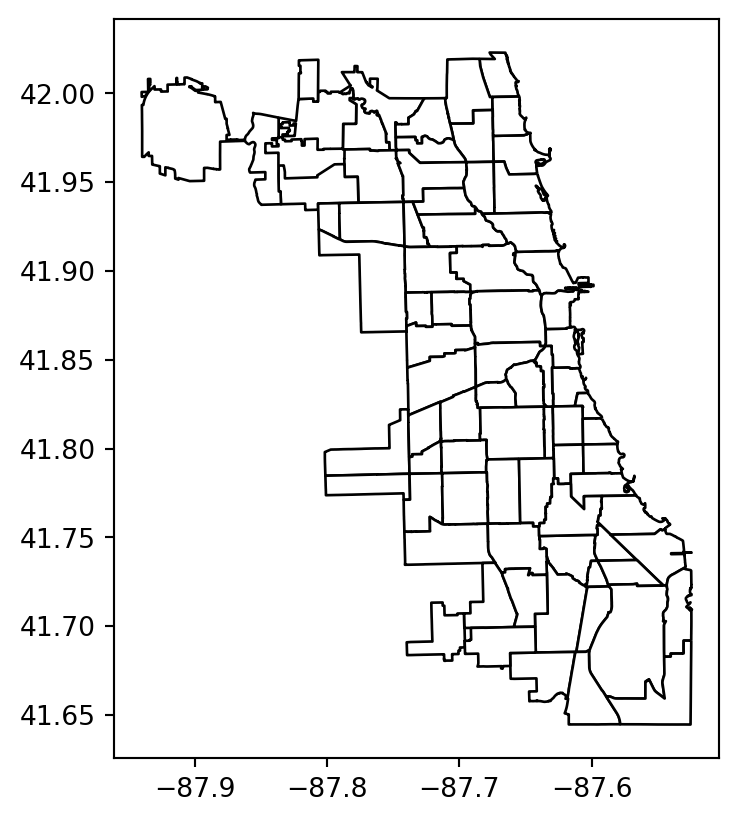
\includegraphics{chap7_files/figure-pdf/cell-13-output-2.pdf}

}

\end{figure}

\begin{Shaded}
\begin{Highlighting}[]
\NormalTok{base }\OperatorTok{=}\NormalTok{ chicago.plot(color}\OperatorTok{=}\StringTok{\textquotesingle{}white\textquotesingle{}}\NormalTok{, edgecolor}\OperatorTok{=}\StringTok{\textquotesingle{}black\textquotesingle{}}\NormalTok{)}
\NormalTok{groceries.plot(ax}\OperatorTok{=}\NormalTok{base, marker}\OperatorTok{=}\StringTok{\textquotesingle{}o\textquotesingle{}}\NormalTok{, color}\OperatorTok{=}\StringTok{\textquotesingle{}red\textquotesingle{}}\NormalTok{, markersize}\OperatorTok{=}\DecValTok{3}\NormalTok{)}\OperatorTok{;}
\end{Highlighting}
\end{Shaded}

\begin{figure}[H]

{\centering 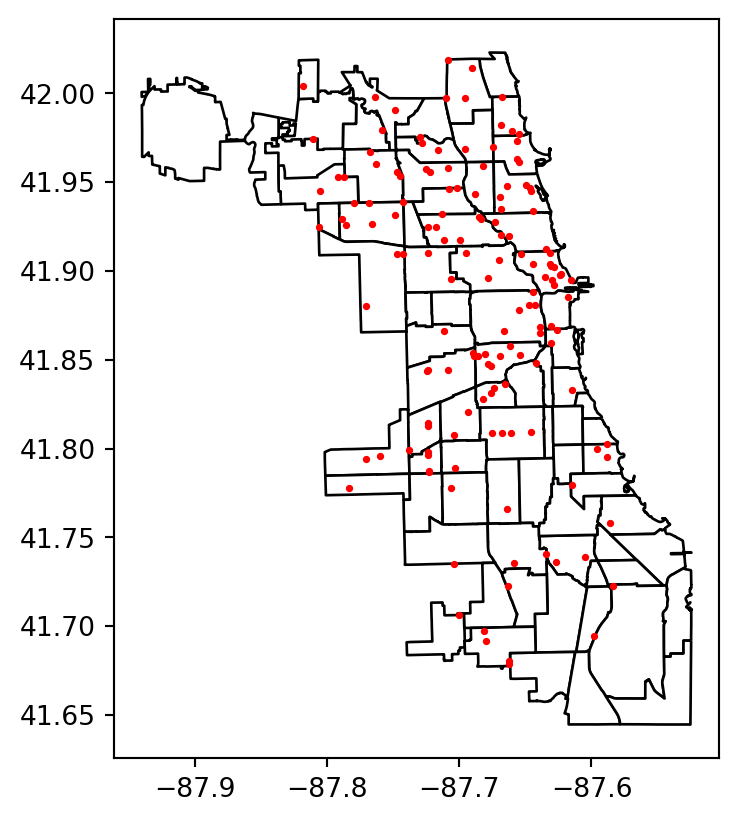
\includegraphics{chap7_files/figure-pdf/cell-14-output-1.pdf}

}

\end{figure}

\hypertarget{reading-external-data}{%
\section{Reading external data}\label{reading-external-data}}

\begin{Shaded}
\begin{Highlighting}[]
\NormalTok{url }\OperatorTok{=} \StringTok{\textquotesingle{}https://raw.githubusercontent.com/jcanalesluna/bcn{-}geodata/master/districtes/districtes.geojson\textquotesingle{}}
\NormalTok{districts }\OperatorTok{=}\NormalTok{ gpd.read\_file(url)}
\NormalTok{districts}
\NormalTok{districts.crs}
\end{Highlighting}
\end{Shaded}

\begin{verbatim}
<Geographic 2D CRS: EPSG:4326>
Name: WGS 84
Axis Info [ellipsoidal]:
- Lat[north]: Geodetic latitude (degree)
- Lon[east]: Geodetic longitude (degree)
Area of Use:
- name: World.
- bounds: (-180.0, -90.0, 180.0, 90.0)
Datum: World Geodetic System 1984 ensemble
- Ellipsoid: WGS 84
- Prime Meridian: Greenwich
\end{verbatim}

\begin{Shaded}
\begin{Highlighting}[]
\NormalTok{districts.plot()}\OperatorTok{;}
\end{Highlighting}
\end{Shaded}

\begin{figure}[H]

{\centering 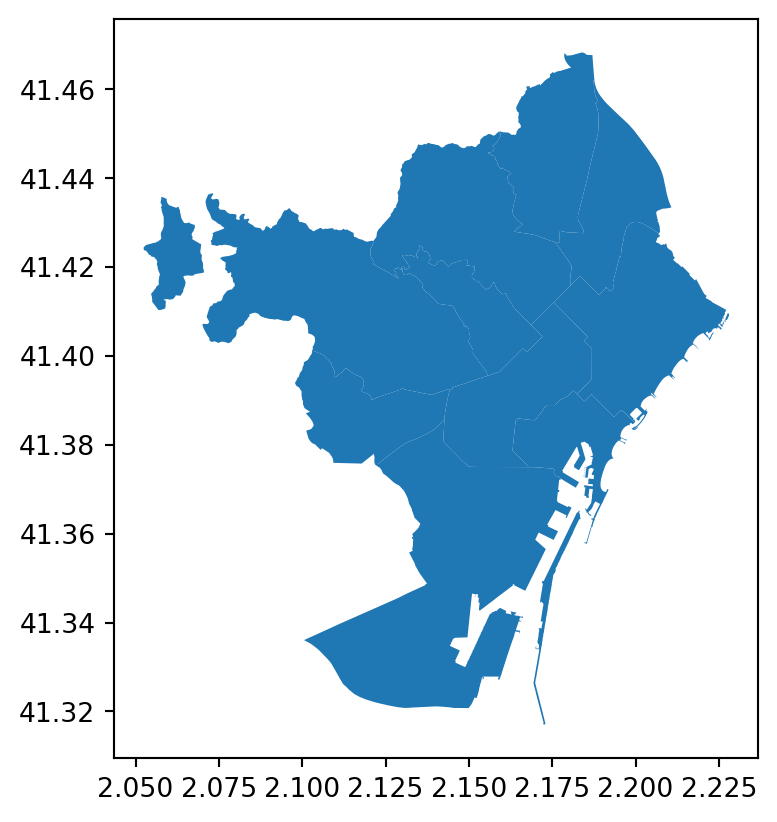
\includegraphics{chap7_files/figure-pdf/cell-16-output-1.pdf}

}

\end{figure}

\bookmarksetup{startatroot}

\hypertarget{references}{%
\chapter*{References}\label{references}}
\addcontentsline{toc}{chapter}{References}

\markboth{References}{References}

\hypertarget{refs}{}
\begin{CSLReferences}{0}{0}
\end{CSLReferences}



\end{document}
